%--------------------------------------------------------------------
%						START PREAMBLE
%--------------------------------------------------------------------

% Two-sided document
\documentclass[11pt]{report}

%Import line number
%\usepackage[]{lineno}
%\linenumbers

%\usepackage[utf8]{inputenc}
%\usepackage{subcaption}
\usepackage{graphicx}
\usepackage[export]{adjustbox}
\graphicspath{ {images/} }
\usepackage{wrapfig}


\usepackage{lipsum}

\usepackage{mdframed}	
\usepackage{setspace}
\usepackage{dirtytalk}

\usepackage{atbegshi}% http://ctan.org/pkg/atbegshi
\AtBeginDocument{\AtBeginShipoutNext{\AtBeginShipoutDiscard}}

\usepackage[
  a4paper,
%  width=160mm,
  top=1in,
  bottom=1in,
  left=1.5in,
  right=1in,
  headsep=10pt,
%  bindingoffset=6mm
  ]{geometry}

\usepackage{comment}

% Caption for figures; To make labels in boldface and set period 
% as separator (e.g. Figure 1. <text>)
\usepackage[
  labelfont=bf,
  labelsep=period,
  size=footnotesize,
  %skip=-5pt,
  font=sf
  ]{caption}	

\usepackage{subcaption}
% For headers and footers
%\usepackage{fancyhdr}
%\pagestyle{fancy}
%\fancyhead{}
%\fancyhead[RE,LO]{\fontsize{10pt}{11pt}\selectfont\leftmark}
%\fancyhead[LE,RO]{\fontsize{10pt}{11pt}\selectfont\rightmark}
%\fancyfoot{}
%\fancyfoot[RE,LO]{\thepage}
%\fancyfoot[LE,RO]{\rightmark}
%\renewcommand{\headrulewidth}{1.5pt}
%\renewcommand{\footrulewidth}{1pt}

%for pdf
\usepackage{pdfpages}
\usepackage{pdflscape}
%----- These are for tables
\usepackage{enumitem}
\usepackage{float}
\usepackage{tabu}
\usepackage{multirow}
\usepackage{array}
\usepackage[table,xcdraw]{xcolor}
\usepackage{tabularray}
\usepackage{threeparttable}
\newcolumntype{L}[1]{>{\raggedright\let\newline\\\arraybackslash\hspace {0pt}}m{#1}}
\newcolumntype{C}[1]{>{\centering\let\newline\\\arraybackslash\hspace{0pt}}m{#1}}
\newcolumntype{R}[1]{>{\raggedleft\let\newline\\\arraybackslash\hspace {0pt}}m{#1}}
\usepackage{tabularx}
\usepackage{makecell}
%-----

% To adjust image positioning
\usepackage[export]{adjustbox}	

\usepackage{mathptmx}
\usepackage{inconsolata}
\usepackage{xr}
\usepackage{setspace}

\usepackage{titlesec}
\titleformat{\chapter}
  {\normalfont\Large\bfseries}
  {\chaptertitlename\ \thechapter }{0pt}{\Large}
\titlespacing*{\chapter}{0pt}{-30pt}{15pt}
\titleformat{\section}
  {\normalfont\large\bfseries}
  {\thesection }{1em}{}

\makeatletter
\def\@makechapterhead#1{%
  \vspace*{-30\p@}%
  {\parindent \z@ \raggedright \normalfont
    \ifnum \c@secnumdepth >\m@ne
      \if@mainmatter
        \Large\bfseries \thechapter.\space
      \fi
    \fi
    \interlinepenalty\@M
    \Large \bfseries #1\par\nobreak
    \vskip 15\p@
  }}
\makeatother

\usepackage{listings}

%settings for my file inputs
\doublespacing
\lstset{basicstyle=\ttfamily, lineskip={-1pt}}
\usepackage{color}
\setlength{\parskip}{1.5pt}
\usepackage{mhchem}
\usepackage{soul}  % For underlines, use \ul{}

\newcommand{\wideunderline}[2][2em]{%
  \underline{\makebox[\ifdim\width>#1\width\else#1\fi]{#2}}%
}

\usepackage{chngcntr} % Changes counter of floats

\renewcommand{\thefootnote}{\fnsymbol{footnote}}
\renewcommand{\contentsname}{Table of Contents}
\renewcommand{\theequation}{Eq \thesection--\arabic{equation}}

\counterwithin{figure}{chapter} %\renewcommand{\thefigure}{\thesection--\arabic{figure}}

\makeatletter
  \renewcommand*\l@figure{\@dottedtocline{1}{0em}{3em}}% 2.3em->3em, 1.5->0
  \renewcommand*\l@table{\@dottedtocline{1}{0em}{2.5em}}% 2.3em->3em, 1.5->0
%  \let\l@table\l@figure
  \renewcommand*\l@lstlisting{\@dottedtocline{1}{0em}{3.5em}}% 2.3em->3em,1.5->0
\makeatother


%setting up tcolorbox
\usepackage[most]{tcolorbox}
\tcbset{
	frame code={}
	center title,
	left=0pt,
	right=0pt,
	top=0pt,
	bottom=0pt,
	colback=gray!25,
        before upper={\singlespacing}
}


\makeatletter
\usepackage{indentfirst}
  \renewcommand*\l@chapter[2]{%
    \addpenalty{-\@highpenalty}%
    \vskip 1.0em \@plus\p@
    \setlength\@tempdima{2.2em}%
    \begingroup
      \parindent \z@ \rightskip \@pnumwidth
      \parfillskip -\@pnumwidth
      \leavevmode \bfseries
      \advance\leftskip\@tempdima
      \hskip -\leftskip
      #1\nobreak\hfil \nobreak\hb@xt@\@pnumwidth{\hss #2}\par
      \penalty\@highpenalty
    \endgroup}
  \renewcommand*\l@section{\@dottedtocline{1}{2em}{1.9em}}
  \renewcommand*\l@subsection{\@dottedtocline{2}{3.7em}{2.5em}}
  \renewcommand*\l@subsubsection{\@dottedtocline{3}{7.0em}{4.1em}}
%  \renewcommand*\l@paragraph{\@dottedtocline{4}{10em}{5em}}
%  \renewcommand*\l@subparagraph{\@dottedtocline{5}{12em}{6em}}
\makeatother

\makeatletter
\renewcommand\subsection{\@startsection{subsection}{2}{\z@}%
                                     {-3.25ex\@plus -1ex \@minus -.2ex}%
                                     {1.5ex \@plus .2ex}%
                                     {\normalfont\bfseries}}
\makeatother

%%for scheme

\usepackage{newfloat}

\DeclareFloatingEnvironment[
  fileext=png,
  listname={List of Scheme},
  name=Scheme,
  placement=tp,
  within=section,% activate it if you want
  chapterlistsgaps=on,% only meaningful when chapters exist
]{scheme}

%\renewcommand{\listfigurename}{List of Figures}
%\renewcommand{\listofscheme}{List of Schemes}
%\renewcommand{\listtablename}{List of Tables}
\renewcommand{\lstlistlistingname}{List of File}
\usepackage{amssymb,amsfonts,amsmath}
\usepackage{gensymb}

% For references and bibliography
\usepackage[
  backend=bibtex,
  sorting=none,
  style=chem-acs,
  citestyle=chem-acs,
  articletitle=true,
  doi=false,
  url=true,
  ]{biblatex}
\usepackage{hyperref}
\usepackage{float}
\hypersetup{
    colorlinks = true,
    linkcolor = black,
    citecolor = black
}

% Adds the bibliography file
\addbibresource{main.bib}


%--------------------------------------------------------------------
%						END PREAMBLE
%--------------------------------------------------------------------

%--------------------------------------------------------------------
%						META INFORMATION
%--------------------------------------------------------------------

% The title page is in a different file

%--------------------------------------------------------------------
%						BEGINNING OF DOCUMENT
%--------------------------------------------------------------------




%\documentclass[11pt, letterpaper]{report}
%\usepackage[margin=1.0in]{geometry}
%\usepackage{graphicx}
%\usepackage{natbib}
%\usepackage{soul}
%\usepackage{xcolor}
%\newcommand{\nel{\textcolor{teal}}}

%\title{\textit{\textbf{Virtual design of benzylisoquinoline alkaloid derivatives as potential therapeutics against two targets in PCOS insulin resistance}}}

%\author{Anatalia Marie M. Bisquera and Rineia Kirsten M. Santos}
%\date{}

\begin{document}

\setcounter{tocdepth}{3}

\begin{singlespace}
	\begin{titlepage}
		\begin{center}
			\fontsize{16pt}{20pt}\selectfont
			
			\vspace*{1cm}
			
			% Title
			{\textbf{Virtual design of benzylisoquinoline alkaloid derivatives as potential therapeutics against two targets in PCOS insulin resistance}}
			
			\vspace*{5.5cm}
			
			% Author
			{\textsc{Anatalia Marie M. Bisquera and Rineia Kirsten M. Santos}}
			
			\vspace*{5cm}
			
			% Affiliation
			{INSTITUTE OF CHEMISTRY\\
				College of Science\\
				University of the Philippines\\
				Diliman, Quezon City}
			
			\vspace{3.5cm}    
			
			MONTH YEAR
		\end{center}
	\end{titlepage}
\end{singlespace}
\pagebreak

\thispagestyle{empty}

{\fontsize{12pt}{15pt}\selectfont

\begin{center}


\includegraphics[height=3cm,center]{Images/University_of_the_Philippines_Manila_Seal.svg.png}

\vspace*{0.2cm}


\noindent\textbf{UNIVERSITY OF THE PHILIPPINES MANILA}

\vspace*{1.5cm}

\noindent\textbf{Bachelor of Science in Biology}

\vspace*{0.2cm}
\noindent\textbf{Anatalia Marie M. Bisquera and Rineia Kirsten M. Santos}

\vspace*{0.2cm}

\noindent\textbf{ \textit{Virtual design of benzylisoquinoline alkaloid derivatives as potential therapeutics against two targets in PCOS insulin resistance}}

\vspace*{2cm}

\noindent Thesis Adviser:

\noindent\textbf{Marla A. Endriga, MPhil, MSc \\ Ricky B. Nellas, Ph.D}

\vspace*{0.2cm}

%\noindent Thesis Co-Adviser:

%\noindent\textbf{\\
%\vspace*{0.2cm}
%Institute of Chemistry\\
%\vspace*{0.2cm}
%University of the Philippines}

\vfill

\noindent Date of Submission\\
\vspace*{5pt}
\noindent January 2024

\vspace*{0.75cm}

\noindent Thesis Classification:\\
\vspace*{5pt}
\noindent\textbf{P}

\vspace*{0.5cm}

\noindent\textit{This thesis is not available to the public. Please ask the library for assistance.}

\end{center}
}
\pagebreak

\tableofcontents
\pagebreak

\chapter{Introduction}
\section{Background of the Study}
 Polycystic ovarian syndrome (PCOS) is a common endocrine, metabolic, and reproductive disorder in women of reproductive age, stemming from an interplay of multiple factors (Diamanti-Kandarakis \& Papavassiliou, 2006; Zhou et al., 2021). Though the precise pathogenesis of PCOS remains obscure, genetics, epigenetics, and the environment have been pinpointed as central to PCOS manifestation. 
 
 At present, an estimate of 6-21\% of women worldwide are afflicted by the syndrome and exhibit a wide range of symptoms at varying degrees (Dunaif, 1997; Zhao et al., 2023). PCOS is characterized by both reproductive and metabolic abnormalities including polycystic ovary morphology, dysfunctional ovulation, and hyperandrogenism alongside insulin resistance (IR) and obesity. Given the heterogeneity of PCOS, four phenotypes have been defined: type A, polycystic ovary, chronic oligo-anovulation and hyperandrogenism; type B, chronic oligo anovulation and hyperandrogenism; type C, polycystic ovary and hyperandrogenism; and type D, polycystic ovary, chronic oligo-anovulation (Dunaif, 1997; Zhao et al., 2023). Additionally, IR—though varying in degree–is present in all phenotypes as 65-95\% of PCOS-affected women regardless of weight suffer from it and compensatory hyperinsulinemia (Zhao et al., 2023). 

Insulin resistance is essentially defined by a decrease in insulin sensitivity. In effect, IR impairs insulin action in its target tissues (adipose, skeletal muscle, liver, ovarian, and uterine tissue), subsequently resulting in compensatory hyperinsulinemia. Specifically, IR hampers insulin-stimulated glucose transport and inhibits lipolysis in adipose tissue; decreases in glucose transport and muscle glycogen synthesis in skeletal muscle; impairs gluconeogenesis suppression but stimulates fatty acid synthesis in liver tissue; and, induces androgen-dependent anovulation in the ovaries and uterus (Hardy et al., 2012; Zhao et al., 2023). In the insulin signal transduction pathway of PCOS women, it has been hypothesized that increased serine phosphorylation and decreased tyrosine phosphorylation of insulin receptors and insulin receptor substrate proteins (IRS) can terminate insulin action (Diamanti-Kandarakis \& Dunaif, 2012). Thus, despite the unaltered affinity of insulin to its receptor, insulin dysfunction may still result due to post-binding defects in insulin signal transduction.

Protein tyrosine phosphatase 1B (PTP1B) normally catalyzes the dephosphorylation of the insulin receptor, thus decreasing insulin-stimulated receptor tyrosine kinase activity. Consequently, an increase of PTP1B activity has been correlated with a loss of insulin signaling (Chen et al., 2010). Similarly, aberrant insulin signaling has also been associated with decreased receptor-mediated insulin substrate tyrosine phosphorylation and an increase of serine phosphorylation due to the action of the inhibitor kappa B kinase (IKK-$\beta$) complex––the second protein target of the present study. Due to the IKK-mediated serine phosphorylation of IRS-1, the protein cannot activate PI3K, thereby halting the subsequent steps in the insulin signaling pathway (Gao et al., 2002).

If left untreated, women with PCOS are more likely to experience adverse pregnancy outcomes such as spontaneous abortions, preterm birth, gestational diabetes mellitus, and pregnancy-induced hypertension (Pattnaik et al., 2022). Furthermore, there is an increased risk of developing type 2 diabetes mellitus, cardiovascular disease, and uterine cancer (Polycystic Ovary Syndrome (PCOS), 2022). 

Oral contraceptives are commonly used to aid in regularizing menstrual periods and mitigating hyperandrogenism, though some studies have found that these agents––especially those containing triphasic progestin––may produce or worsen IR (Dunaif, 1997). Metformin, on the other hand, suppresses hepatic glucose production and improves insulin sensitivity by mediating weight loss. Nevertheless, it does not help manage androgen levels nor does it alter insulin action itself (Dunaif, 1997; Huang et al., 2016; Zhao et al.,  2023). Thiazolidinediones (TZDs) like troglitazone and pioglitazone are true insulin sensitizers that target peroxisome proliferator activated receptor gamma (PPAR-$\gamma$), which mediates insulin activity. Unlike metformin, however, TZDs do so without altering body weight while also lowering androgen, estrogen, and luteinizing hormone levels in PCOS (Huang et al., 2016; Zhao et al., 2023). Similarly, myo-inositol, a sugar-alcohol supplement, has been observed to exhibit insulin sensitization efficiency while also promoting ovulation (Zhao et al.,  2023). 

Lastly, berberine, a benzylisoquinoline alkaloid derivative isolated from Traditional Chinese medicinal herbs, is known to alleviate metabolic disorders. Berberine itself participates in several insulin signaling pathways (i.e., PPAR, MAPK, AMPK), making it a novel PCOS treatment (Zhao et al., 2023). In relation to the aforementioned protein targets, BRR has the potential to bind PTP1B, inhibiting its catalytic activity which consequently enhances the phosphorylation of insulin receptor and insulin receptor substrate-1 (IRS-1) in 3T2-L1 adipocytes (Zhang et al., 2021). Furthermore, a previous study involving gestational diabetes mellitus (GDM) rats found that the binding of BRR to IKK-$\beta$ results in decreased IR due to the modulation of different signaling pathways in the liver (Li et al., 2022). In effect, by activating insulin signaling pathways and promoting the utilization of glucose, berberine and perhaps its functional derivatives may have the potential to manage IR that exacerbates PCOS progression.

\section{Statement of the Problem}
What benzylisoquinoline alkaloid derivatives have the greatest binding affinities to PTP1B and IKK-$\beta$ and possess suitable chemical properties for drug development, thus becoming effective inhibitors towards insulin resistance?  

\section{Research Objectives}
The aim of the present study is to identify and design benzylisoquinoline alkaloid-based drug leads targeting protein tyrosine phosphatase 1B (PTP1B) and inhibitor kappaB kinase (IKK) complexes as treatments for PCOS insulin resistance. 

Specifically, the researchers aim to: 
\begin{itemize}
     \item Identify benzylisoquinoline alkaloid derivatives that effectively bind to PTP1B and IKK-$\beta$ via structure-based virtual screening.
     \item Determine the binding affinity of top-hit benzylisoquinoline alkaloid derivatives to PTP1B and IKK-$\beta$ respectively through molecular docking. 
    \item Optimize benzylisoquinoline alkaloid-based ligand using QSAR results.
    \item Describe protein-ligand interactions between initial top binding compounds and modified benzylisoquinoline alkaloid ligands with the PTP1B and IKK-$\beta$ through computer-aided visualization. 
    \item Evaluate the top candidate ligands based on physicochemical and pharmacokinetic properties using ADMETox assessments.
    \item Determine if best-binding modified benzylisoquinoline alkaloids may be naturally sourced (i.e., from plants, microorganisms, animals, etc.).
\end{itemize}

\section{Significance of the Study}
This study will provide essential baseline information on the viability of berberine derivatives as a form of treatment for PCOS insulin resistance by binding specifically to PTP1B and IKK. Moreover, the availability of information about berberine’s effect on PCOS pathways remains scarce as it has only gained interest in the field recently. Data generated throughout the study will be able to supplement existing evidence that the intake of berberine decreases insulin resistance and improves the overall menstrual patterns in infertile PCOS women. 

\section{Scope and Limitations}
The study aims to identify the most promising benzylisoquinoline alkaloid derivative with high potential for therapeutic effects against IR manifested in PCOS women when bound separately to PTP1B and IKK target proteins. Computational analysis tools, such as MTiOpenScreen web server, AutoDock Tools, GROMACS, MarvinSketch,3DQSAR, LigPlot+, and ADMETox will be employed to design benzylisoquinoline alkaloid-based ligands and determine the key interactions that occur in the generated models. \textit{In vitro} and \textit{in vivo} experiments are beyond the scope of this study.
\pagebreak

\chapter{Review of Related Literature}
\section{PCOS}

PCOS is a multifaceted endocrine, metabolic, and reproductive disorder affecting a significant number of reproductive-aged women globally. Characteristic manifestations include hyperandrogenism, oligo-anovulation, polycystic ovarian morphology, and insulin resistance via preferential abdominal fat accumulation (Dumesic et al., 2022). 

Four phenotypes have been identified which group the multifaceted symptoms of the disorder when observed via ultrasound (See \ref{tab:Phenotypes}) (Khan et al., 2017). Phenotypes A and B are the classic representation of PCOS and are characterized by oligoanovulation and hyperandrogenism, with type A further possessing multiple polycystic ovaries. Given that the two differ solely in terms of ovarian morphology, endocrine or metabolic differences do not exist. Phenotype C (ovulatory PCOS) is characterized by polycystic ovaries with the occurrence of routine menses and hyperandrogenism. Lastly, phenotype D (Nonhyperandrogenic PCOS) is marked by polycystic ovaries, oligoanovulation, and the lack of hyperandrogenism. The NIH diagnostic criteria recognize phenotypes A and B, the Rotterdam criteria accept all four phenotypic groups, and the AES classification takes into account the first three phenotypic classes only (Lujan et al., 2008; Khan et al., 2017). Proper classification of the phenotypes is crucial for the correct diagnosis of the disease and implementation of suitable treatment strategies. 

% \usepackage{tabularray}
\begin{table}
    \centering
    \caption{PCOS Phenotypes and Corresponding Manifestations}
    \label{tab:Phenotypes}
\begin{tblr}{
  row{odd} = {c},
  row{2} = {c},
  row{4} = {c},
  cell{2}{2} = {r=2}{},
  hline{1-2,6} = {-}{},
}
\textbf{Phenotype} & \textbf{Type}       & \textbf{Manifestations}                                \\
A                  & Classical           & Hyperandrogenism, oligoanovulation, polycystic ovaries \\
B                  &                     & Hyperandrogenism and oligoanovulaiton                  \\
C                  & Ovulatory           & Hyperandrogenism and polycystic ovaries                \\
D                  & Nonhyperandrogenic~ & Oligoanovulation and polycystic ovaries                \\
                   &                     &                                                        
\end{tblr}
\end{table}

\section{Multifaceted Pathology of PCOS}

PCOS patients may experience adverse manifestations due to the presence of excess male sex hormones such as hirsutism, androgenic alopecia, and acne–commonly known as hyperandrogenism (Wang \& Li, 2023). The CYP11A1 gene mainly functions in the catalysis of cholesterol to pregnenolone which is necessary in steroidogenesis or the synthesis of sex hormones. A promoter pentanucleotide repeat (tttta)n polymorphism in this gene is often associated with elevated androgen levels and is considered a risk molecular marker for PCOS. A case-control study that evaluated the PCOS susceptibility of CYP11A1 polymorphism from extracted, amplified, and genotyped DNA of 267 PCOS patients and 275 controls from South India found that alleles with repeats above 8 exhibited a three-fold risk for PCOS susceptibility as compared to the controls (Reddy et al., 2014). 

Another gene involved in steroidogenesis is CYP17A1 which converts pregnenolone and progesterone into 17-hydroxypregnenolone and 17-hydroxyprogesterone and inverts these steroids into dehydroepiandrosterone (DHEA) and $\Delta$4-Androstendione ($\Delta$4A), which is catalyzed by the P450c17 enzyme (Panda et al., 2016). Polymorphism in this gene was found to increase body weight, IR, and excessive lipid in a study conducted on the Chilean population (Ajmal et al., 2019). Moreover, the enzymatic activity of P450c17 was observed to increase the abundance of ovary theca cells in PCOS women (Panda et al., 2016).

Abnormal levels of gonadotropin secretion are another manifestation of PCOS that is influenced by an elevated level of luteinizing hormones (LH) and low levels of follicle-stimulating hormone (FSH). Decreased levels of FSH increase the risk of infertility due to the failure of the follicle to mature and consequently release eggs. Follicular cysts emerge in follicles that fail to ovulate and are characterized by an increased abundance of follicular fluid and the absence of an oocyte (Ndefo et al., 2013). 

Metabolic aberrations due to excess androgen are also notable pathologic factors of PCOS. Specifically, type 2 diabetes or glucose intolerance has been shown to have higher occurrences in PCOS women despite the absence of obesity (Christakou \& Diamanti-Kandarakis, 2008). However, more complex metabolic phenotypes may arise in the presence of obesity, which accounts for approximately 50\% of PCOS women, due to the added interactions with metabolic abnormalities. Ehrmann et al. (1999) found that 45\% of 122 women with clinical and hormonal evidence of PCOS showed abnormal levels of glucose tolerance. Additionally, evidence has shown the increased pathogenesis of type 2 diabetes mellitus in obese individuals due to the stimulation of IR (Wondmkun, 2020).

\section{Insulin Resistance and PCOS}
IR has been identified as the predominant manifestation among women diagnosed with PCOS due to the aberrant functioning of one or more elements of the insulin transduction pathway (Zhao et al., 2023). Within the context of PCOS, the dysfunction of this molecular process effectively decreases tissue sensitivity to insulin, resulting in impaired insulin-stimulated glucose transport and inhibited lipolysis in adipose tissue; reduced insulin-mediated glucose processing in skeletal muscle; impaired gluconeogenesis suppression but stimulated fatty acid synthesis in liver tissue; and, androgen-dependent anovulation in the ovaries and uterus (Hardy et al., 2012; Zhao et al., 2023).

Under physiologically normal conditions, insulin binds to its receptor, activating a tyrosine kinase. This leads to further autophosphorylation of the insulin receptor beta subunit, which in turn phosphorylates insulin receptor substrates (IRS) that serve as docking sites for phosphoinositide 3-kinases (PI3K). Activation of PI3K directly enables the translocation GLUT-4 transporters to the cell surface which facilitates insulin-dependent glucose uptake by cells (See \ref{fig:InsulinPath}). Additionally, activated PI3K leads to the phosphorylation of protein kinase B (PKB or Akt), which subsequently phosphorylates glycogen synthase kinase-3 (GSK3), effectively inactivating it. Due to GSK3 inactivation, glycogen synthase is activated to catalyze glycogenesis (Diamanti-Kandarakis \& Papavassiliou, 2006). 

\begin{figure} 
            \centering
            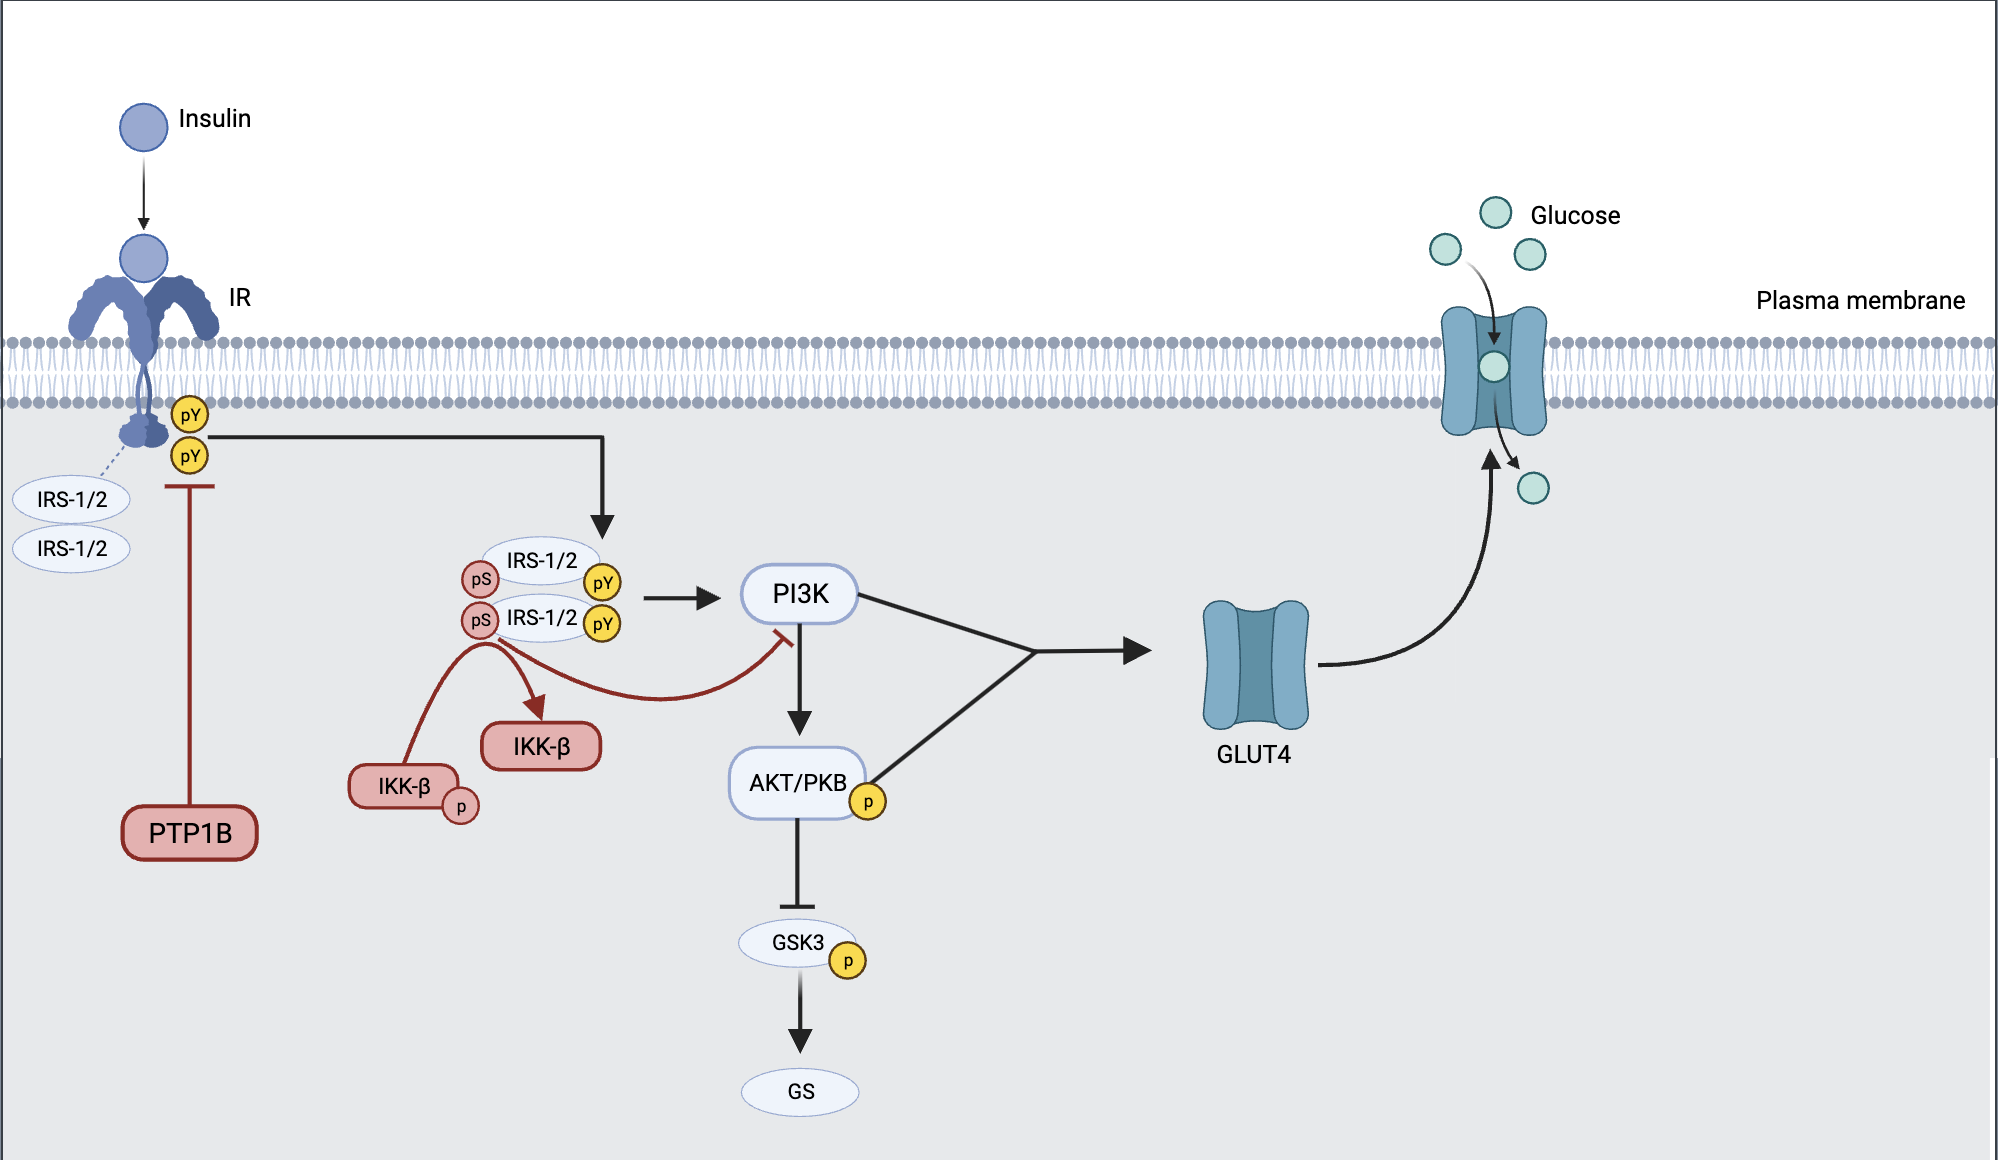
\includegraphics[width=1\linewidth]{Images/pathway.png}
            \caption{Insulin Signal Transduction Pathway}
            \label{fig:InsulinPath}
        \end{figure}

\subsection{PCOS Aberrant Insulin Pathway}
However, women with PCOS are unable to perform this standard mechanism likely due to multiple irregularities. In the insulin signal transduction pathway of PCOS women, it has been suggested that increased serine phosphorylation and decreased tyrosine phosphorylation of insulin receptors and insulin receptor substrate proteins (IRS) can terminate insulin action (Diamanti-Kandarakis \& Dunaif, 2012). Thus, despite the unaltered affinity of insulin to its receptor, insulin dysfunction may still result due to post-binding defects in insulin signal transduction. 

To illustrate, a study found that 50\% of PCOS-cultured skin fibroblasts presented decreased insulin receptor autophosphorylation due to decreased insulin-dependent tyrosine phosphorylation and increased insulin-independent receptor serine phosphorylation. The latter is known to inhibit receptor tyrosine kinase activity, thereby terminating the insulin-signaling pathway in its early steps. Furthermore, this abnormality has also been observed in insulin receptors isolated from classic insulin target tissues, specifically skeletal muscle. This trend of increased insulin-independent serine phosphorylation seems to be unique to PCOS as this tendency is not observed in other insulin disorders like non-insulin-dependent diabetes mellitus. 

On the other hand, the other 50\% of skin fibroblasts from PCOS women did not exhibit the abnormality in insulin receptor phosphorylation. However, there was a decrease in muscle PI3K activation during insulin infusion, and thus reduced translocation of GLUT-4 to the cell surface. Additionally, a recent study found elevated phosphorylation residues on IRS-1 and IRS-2, resulting in lower insulin-mediated IRS-1-related PI3K activation due to targeted IRS-1 destruction. In conjunction with these findings, other studies of skeletal muscle have demonstrated reduced phosphorylation of PKB and the PKB substrate. As such, it has been hypothesized that a defect downstream of insulin receptor signaling, namely, phosphorylation of IRS-1 or activation of PI3K is responsible (Dunaif et al. 1995 as cited in Dunaif, 1997).

\subsection{Protein tyrosine phosphatase 1B in PCOS}
Human protein tyrosine phosphatase 1B (PTP1B, PDB ID: \href{https://www.rcsb.org/structure/4I8N}{4I8N}) is a 435 amino acid-long, 49 kDa peripheral membrane protein of the endoplasmic reticulum encoded by the PTPN1 gene. It is an asymmetric monomer of the non-receptor protein tyrosine phosphatases (non-receptor class I subfamily), composed of an N-terminal catalytic domain (1-300), a regulatory domain (301-400), and a C-terminal domain (400-435). Specifically, binding sites include residue 181, 215-221, and 262, while the active site is marked on a cysteine residue at position 215 (Bateman et al., 2022; Liu et al., 2022)

The N-terminal catalytic domain is composed of eight $\alpha$-helices and twelve $\beta$-strands (see \ref{fig:4i8n}).  It is regulated by post-translational modifications such as the phosphorylation of serine and tyrosine residues and the oxidation of the catalytic cysteine (Cys215). For instance, phosphorylation of Ser50 decreases PTP1B activity, thus hindering PTP1B-mediated dephosphorylation of the insulin receptor. Conversely, phosphorylation of Tyr66 in response to insulin stimulation leads to the negative regulation of the insulin pathway. The catalytic cysteine, however, was identified to modulate the degree and duration of phosphotyrosine-dependent signaling wherein its oxidation would terminate PTP1B activity transiently or permanently depending on its oxidized form (Liu et al., 2022).  

    \begin{figure} 
        \centering
        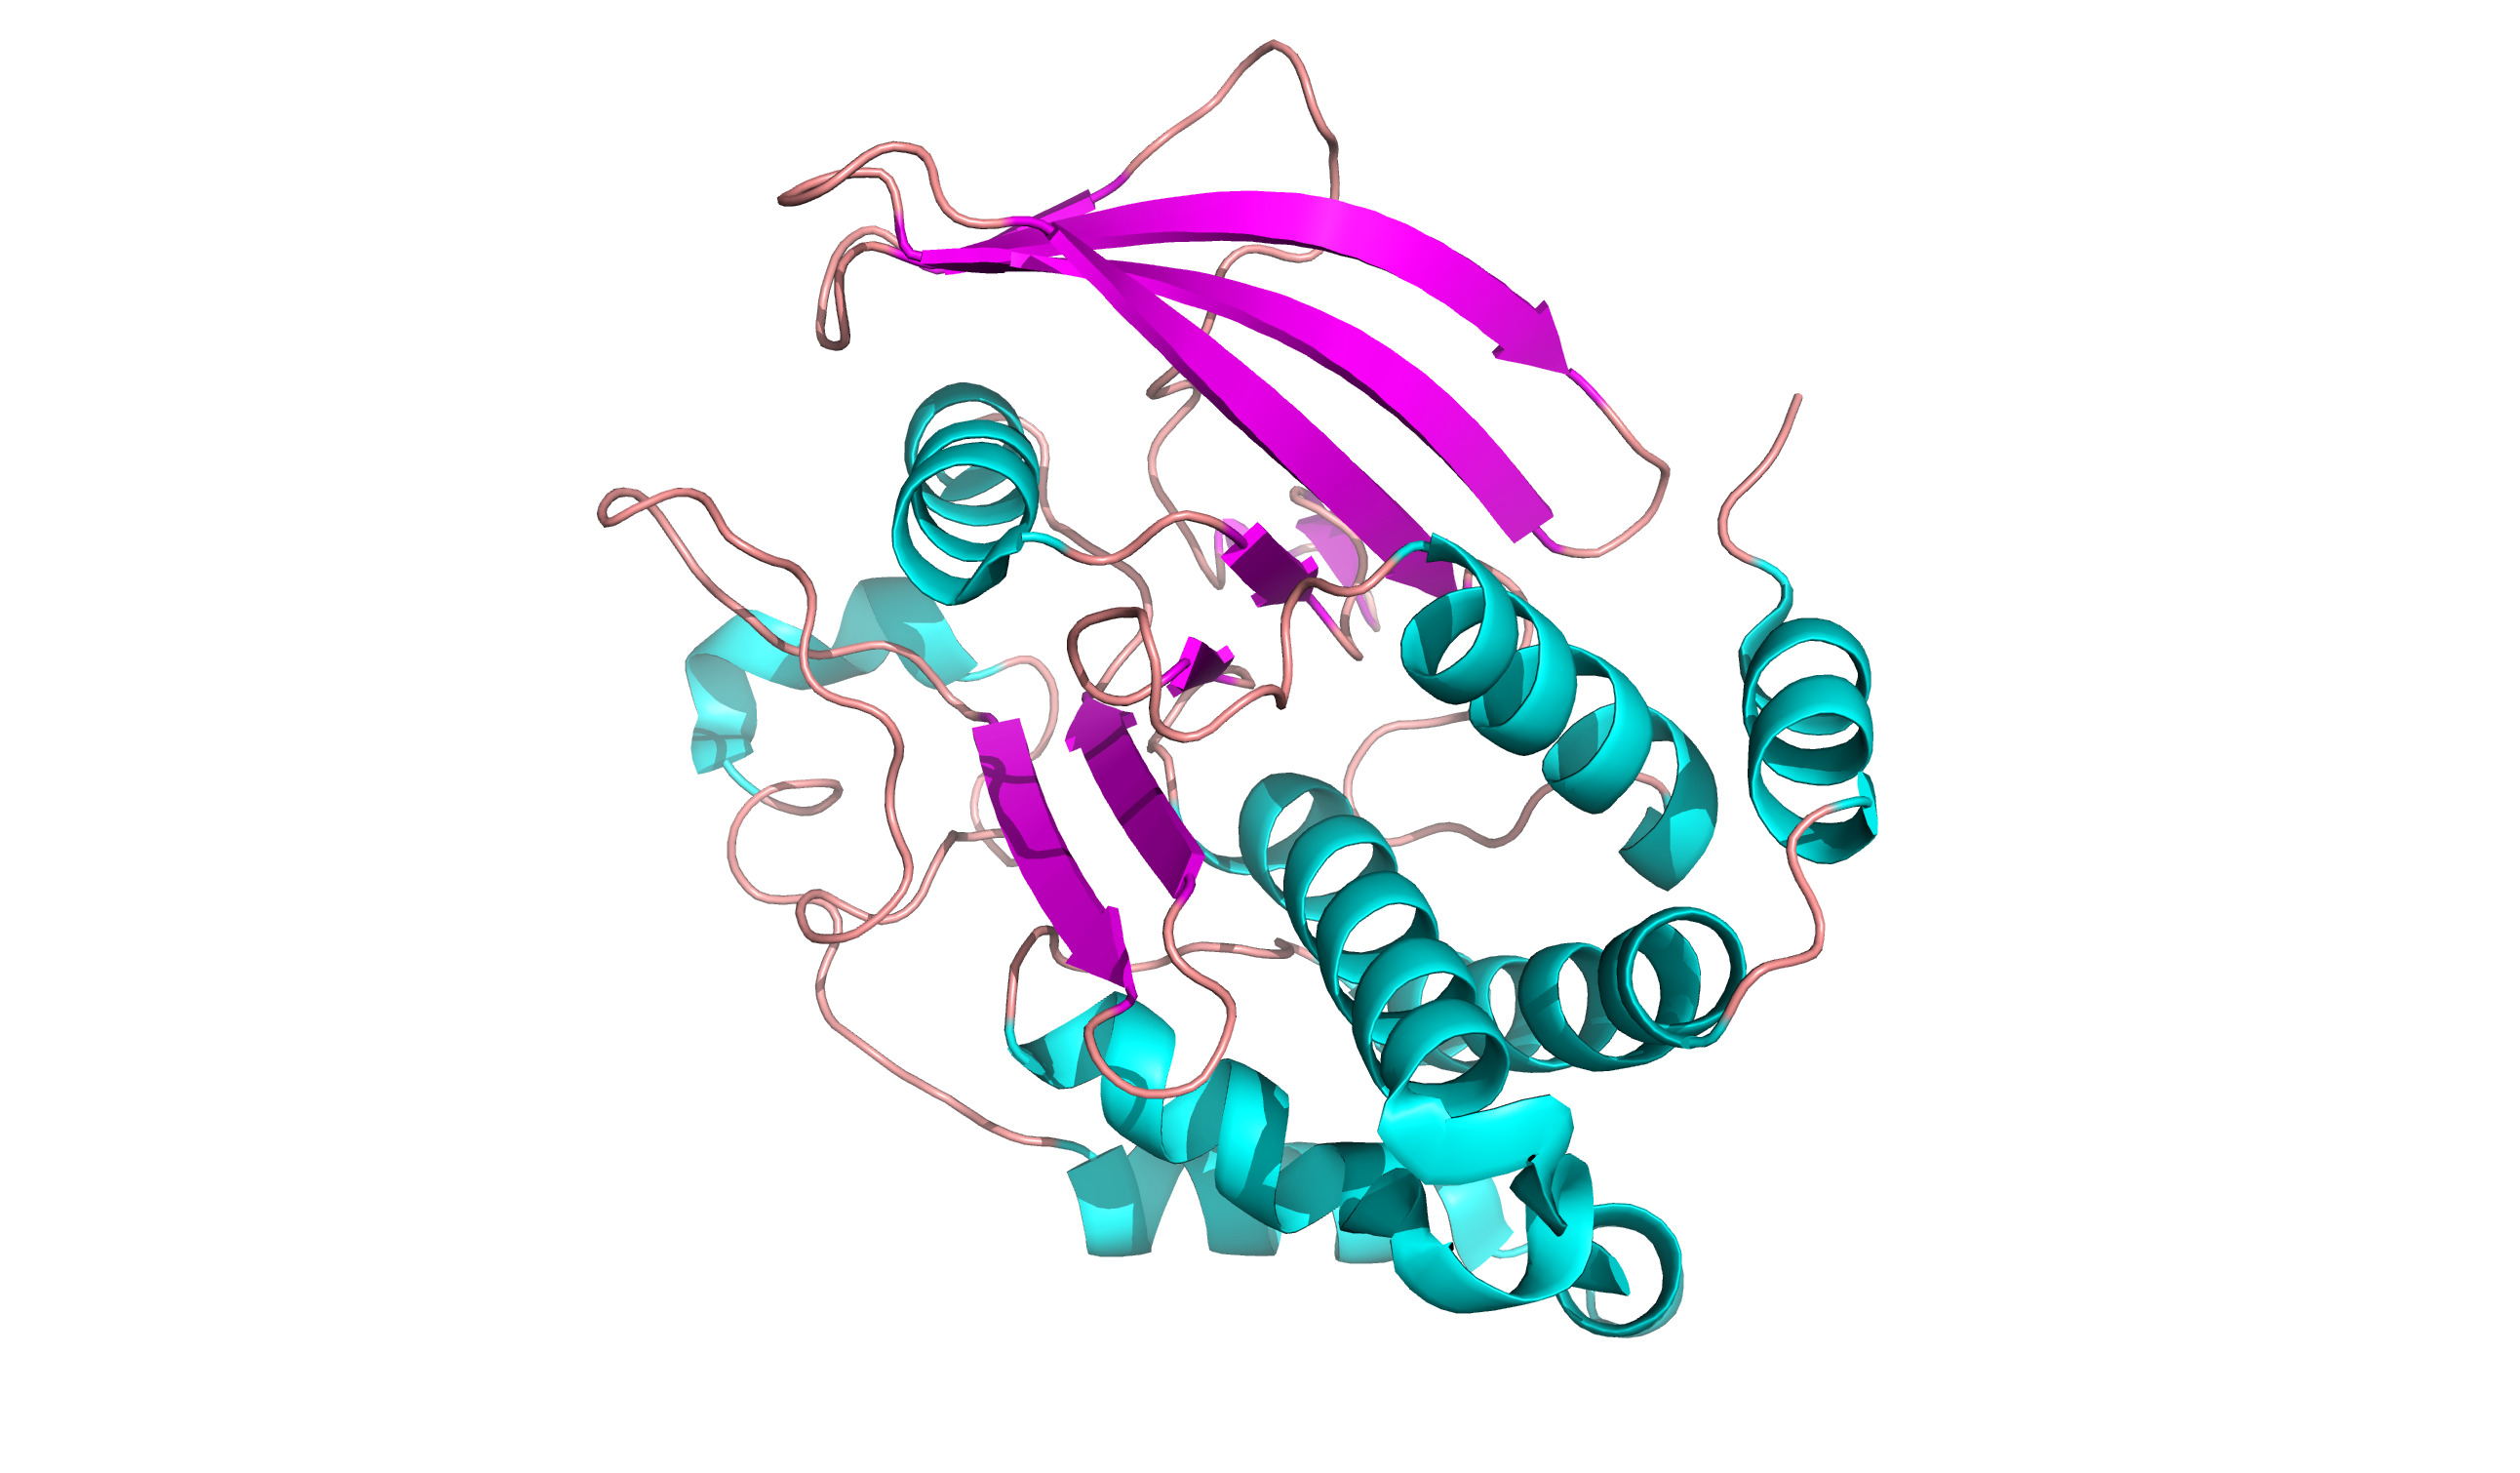
\includegraphics[width=1\linewidth]{Images/4i8n_ss.png}
        \caption{X-ray crystallographic structure of PTP1B}
        \label{fig:4i8n}
    \end{figure}

The regulatory domain is proline-rich and functions as an interaction site for Src homology 3 domain-containing proteins. Substituting crucial proline residues inhibits PTP1B from binding to and activating Src, but it does not impact its dephosphorylating function on insulin receptors (Liu et al., 2022). With this, it is crucial to signal transduction mechanisms of insulin, leptin, growth hormone, and endoplasmic reticulum stress (Delibegović \& Mody, 2013). 

Within the context of insulin resistance specifically, PTP1B is a negative regulator of insulin signaling and normally catalyzes the dephosphorylation of the insulin receptor, thus reducing insulin-stimulated receptor tyrosine kinase activity (See \ref{fig:InsulinPath}). Consequently, an increase of PTP1B activity has been correlated with a loss of insulin signaling (Chen et al., 2010). Indeed, studies have found that PTP1B knockout mice showcased enhanced insulin sensitivity due to increased insulin receptor and IRS-1 tyrosine phosphorylation (Galić et al., 2005). In line with these observations, inhibiting the catalytic action of PTP1B may effectively increase the tyrosine phosphorylation of insulin receptors and IRS-1.  

\subsection{Inhibitor kappa B kinase in PCOS}
Human inhibitor kappa B kinase (IKK-$\beta$, PDB ID: \href{https://www.rcsb.org/structure/4KIK}{4KIK}) is a key regulator of the NF-$\kappa$B signaling pathway (see \ref{fig:4kik}). Comprising the IKK multiprotein complex together with IKK-$\alpha$ and NEMO, IKK-$\beta$ contains an N-terminal kinase domain (15-308), a leucine zipper region (458-479), a helix-loop-helix region (603-642), NEMO binding domain (737-742), and a ubiquitin-like domain (ULD) domain which is unique to its kind and is necessary for NF-$\kappa$B activation (May et al., 2004; Liu et al., 2013). 

        
Among the two principal catalytic subunits, IKK-$\beta$ regulates the classical canonical pathway of NF-$\kappa$B signaling which underlies immune and inflammatory response functions (May et al., 2004). The classical pathway is activated by pro-inflammatory stimuli (i.e., TNF-$\alpha$ and interleukin-1 (IL-1) through the toll-like receptors (TLRs) and triggers the recruitment of TNF receptor-associated factors (TRAFs) (Gamble et al., 2012). This then facilitates the recruitment of key enzymes such as MAP or ERK kinase kinase 3 (MEKK3) and transforming growth factor-$\beta$ (TGF-$\beta$)-activated kinase 1 (TAK1) that specifically activate IKK$\beta$ through phosphorylation at Ser 177 and Ser 181 within the activation loop. Once activated, IKK$\beta$ phosphorylates I$\kappa$B$\alpha$ (Ser 32 and Ser 36) or I$\kappa$B$\beta$ (Ser 19 and Ser 23), triggering polyubiquitination and subsequent proteasomal degradation of I$\kappa$B. The consequent liberation of NF-$\kappa$B enables its nuclear translocation and binding to gene promoter regions, thus initiating transcriptional activation (Gamble et al., 2012).

    \begin{figure} 
        \centering
        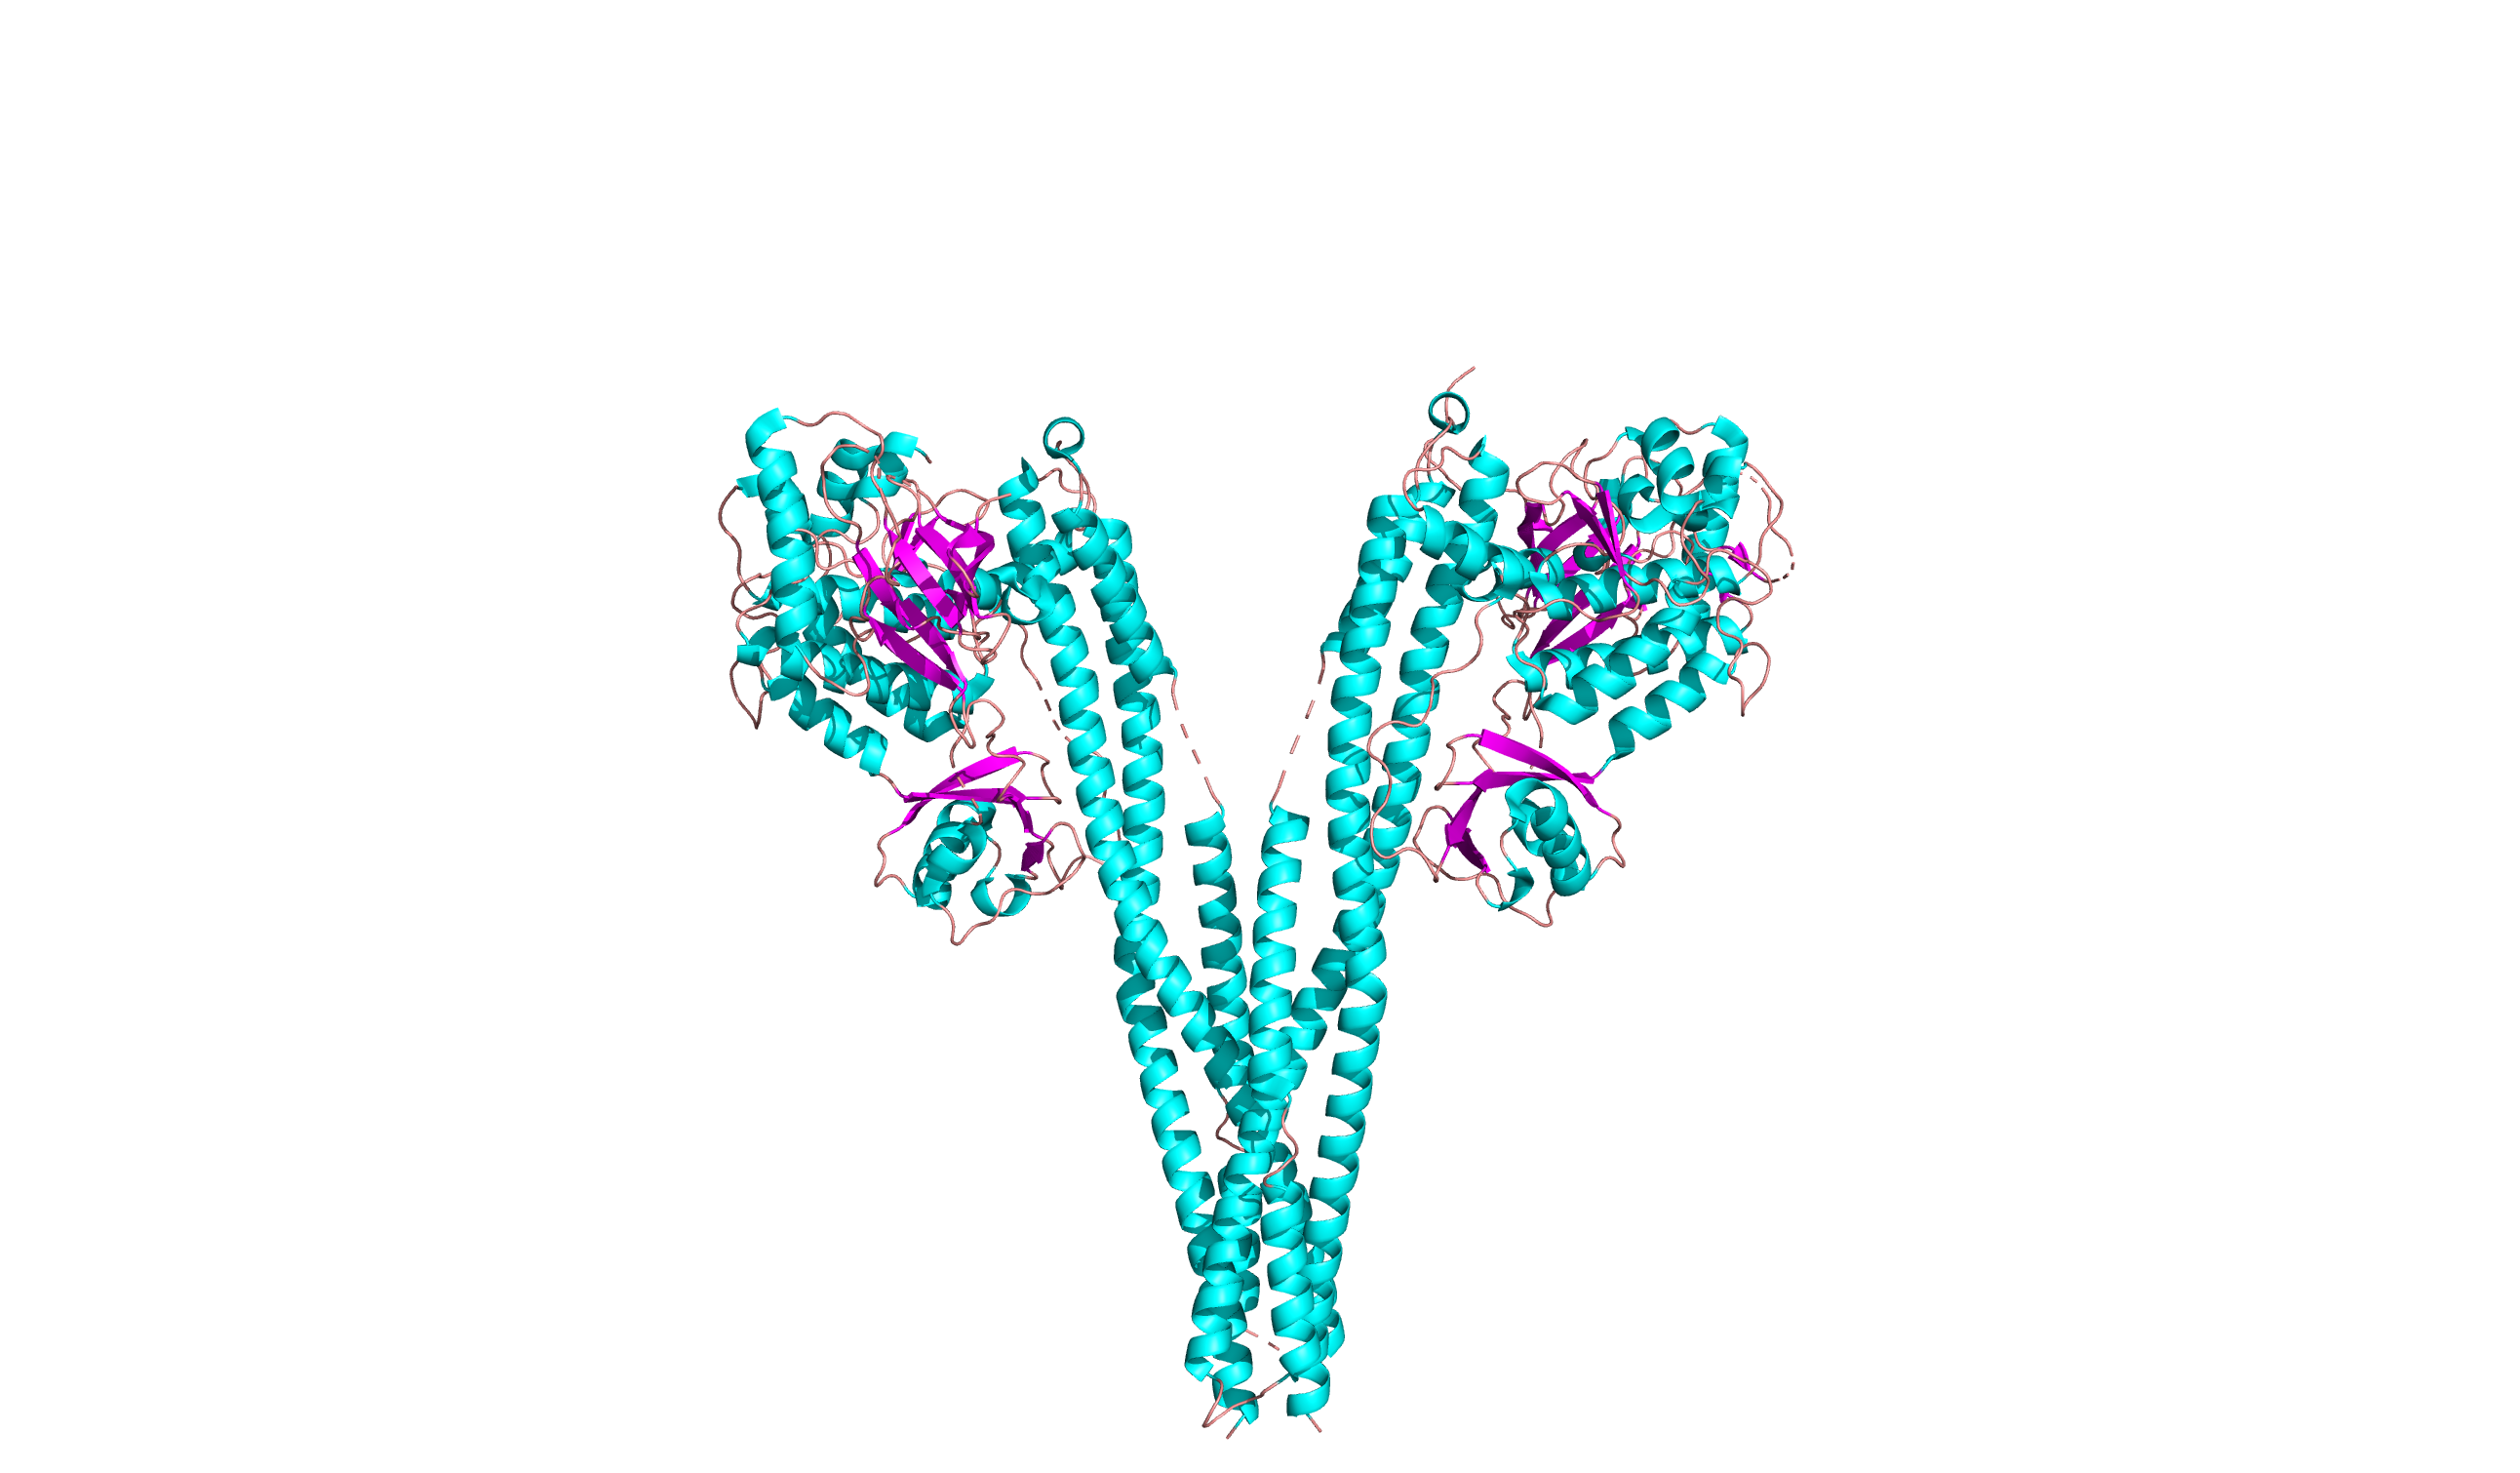
\includegraphics[width=1\linewidth]{Images/4kik_ss.png}
        \caption{X-ray crystallographic structure of IKK-$\beta$}
        \label{fig:4kik}
    \end{figure}

Under normal circumstances, NF-$\kappa$B is sequestered in the cytoplasm through its association with I$\kappa$B proteins, preventing its nuclear localization (Chen et al., 2015). The deficiency of IKK-$\beta$ in adipose cells was shown to prevent the free fatty acid-induced expression of target genes that encode inflammatory mediators (i.e., TNF-$\alpha$ and IL-6) while its activation suppressed the expression of anti-inflammatory cytokines (i.e., leptin and adiponectin) (Jiao et al., 2011). 

This underscores the relevance of the IKK-$\beta$/NF-$\kappa$B pathway to overall IR since the elimination of IKK-$\beta$ and inhibition of NF-$\kappa$B results in improved glucose tolerance and insulin sensitivity (Chen et al., 2015). In instances of insulin resistance, serine phosphorylation of IRS-1 has been correlated with the activation of the IKK-$\beta$ complex (Gao et al., 2002; Liu et al., 2012). Gao et al. (2002) found that serine phosphorylation of IRS-1 at Ser(312) in response to TNF-$\alpha$ was reduced in cells treated with IKK inhibitor 15 deoxy-prostaglandin and in cells from IKK-knockout mice. Thus, IRS-1 is suggested to be a direct substrate of IKK-$\beta$, which results in IRS-1 serine phosphorylation and, ultimately, impairment of the PI3K insulin signal transduction pathway (See \ref{fig:InsulinPath}). Consequently, inhibiting the binding between IRS-1 and IKK-$\beta$ may mitigate insulin resistance initially caused by the early-stage termination of the insulin transduction pathway.


\section{Current Treatments for PCOS Insulin Resistance}

Generally, treatment for PCOS varies due to the heterogeneity of its manifestation. The appropriate treatment depends on the individual’s PCOS phenotype as therapeutics for certain symptoms may exacerbate others. For instance, oral contraceptives are widely used to treat menstrual irregularities and hyperandrogenism. However, triphasic progestin-based oral contraceptives have been seen to worsen insulin resistance. To avoid this, one may opt for norethindrone-only contraceptives as an alternative (Dunaif, 1997).  

Hence, to specifically address insulin resistance, metformin, myo-inositol, and thiazolidinediones have commonly been prescribed as well as the novel berberine supplement isolated from traditional Chinese medicine (See Table \ref{tab:Treatment}). 

% \usepackage{tabularray}
\begin{table} [h]
    \centering
    \caption{PCOS Insulin Resistance Treatment Options}
    \label{tab:Treatment}
\noindent\begin{minipage}{\linewidth}
\resizebox{\linewidth}{!}{%
\begin{tblr}{
  row{1} = {c},
  cell{2}{1} = {r=4}{c},
  cell{2}{2} = {r=4}{c},
  cell{2}{4} = {r=2}{},
  cell{4}{4} = {r=2}{},
  cell{6}{1} = {c},
  cell{6}{2} = {c},
  cell{7}{1} = {r=3}{c},
  cell{7}{2} = {r=3}{c},
  cell{7}{4} = {r=3}{},
  cell{10}{1} = {r=3}{c},
  cell{10}{2} = {r=3}{c},
  cell{10}{4} = {r=3}{},
  hline{1-2,13} = {-}{},
}
\textbf{Treatment} & \textbf{Benefits} & \textbf{Mechanism} & \textbf{Side-Effects~}\\
\textbf{Metformin} & Insulin sensitization & Suppress hepatic glucose synthesis & {Vitamin B12 Deficiency \\(breathlessness, fatigue,  lethargy)}\\
 &  & Improve translocation of GLUT-1 and/or GLUT-4~ & \\
 &  & Activate AMPK to promote glucose uptake~ & Lactic acidosis (severe overdose)\\
 &  & Promote adiponectin in endometrial tissues & \\
\textbf{Myo-inositol} & Insulin sensitization~ & {Activation of PI3K/AKT pathway, activating \\glycogen synthase and GLUT-4 translocation~} & {Nausea, diarrhea, abdominal pain, \\fatigue, headache, dizziness~}\\
\textbf{TZDs} & Insulin sensitization & {Act on PPAR-γ to stimulate insulin activity \\through post-insulin receptor mechanism~} & {Hepatotoxicity: severe reversible liver \\failure, liver injury, and death}\\
 &  & {PTP1B inhibitor to promote tyrosine phosphorylation \\of insulin receptor and IRS-1} & \\
 &  & {IKK-β inhibitors to inhibit serine phosphorylation \\of IRS-1} & \\
\textbf{Berberine}~ & Insulin sensitization & Activate AMPK to promote glucose uptake~ & {Allergic reactions, drug-drug interactions, \\and toxicity consequences (altered liver \\function, gastric issues, hemorrhagic \\inflammation, hepato- and hematotoxicity, \\damage to immune cells)}\\
 &  & {PTP1B inhibitor to promote tyrosine phosphorylation \\of insulin receptor and IRS-1} & \\
 &  & IKK-β inhibitor to inhibit serine phosphorylation of IRS-1 & 
\end{tblr}
}
\end{minipage}
\end{table}

Metformin is the most widespread therapeutic prescribed to those suffering from insulin resistance due to its ability to suppress glucose synthesis in the liver and increase insulin sensitivity via weight loss (Dunaif, 1997). Metformin acts as an insulin sensitizer by improving the translocation of glucose transporters, GLUT-1 and/or GLUT-4 to cell membranes, activating the  5'-adenosine monophosphate-activated protein kinase (AMPK) signaling pathway responsible for promoting glucose uptake, and promotes the use of insulin-sensitizing molecules like adiponectin in endometrial tissues (Zhao et al., 2023). 

Although metformin has its benefits, its long-term use can result in vitamin B12 deficiency. Consequently, B12 supplementation may be necessary to mitigate symptoms of the deficit such as breathlessness, fatigue, and lethargy (NHS, 2022). Furthermore, it may–though rarely–cause metformin-associated lactic acidosis in cases of severe overdose (Dyatlova, 2023).


Similarly, the sugar-alcohol supplement myo-inositol, has been observed to aid in insulin sensitivity (Zhao et al., 2023). After insulin-dependent stimulation and activation of phosphatidyl-inositol-specific phospholipase C, the liver releases inositol phosphoglycans that contain either myo-inositol or d-chiro-inositol which eventually activate glycogen synthase through the PI3K/AKT pathway. Ultimately, this inactivates GSK3, enhances glycogen synthase and GLUT-4 translocation, and glucose uptake (Merviel et al., 2021).  

On the other hand, thiazolidinediones (TZDs) are true insulin sensitizers as they act on the nuclear receptor, peroxisome proliferator-activated receptor gamma (PPAR-$\gamma$), thus enhancing insulin activity through a post-insulin receptor mechanism (Huang et al., 2016; Zhao et al., 2023). Moreover, TZDs are PTP1B inhibitors and irreversible allosteric IKK-$\beta$ inhibitors, thus promoting tyrosine phosphorylation of IR and IRS-1 and inhibiting IRS-1 serine phosphorylation respectively (Verma et al., 2019; Elkamhawy et al., 2020). TZDs thus improve insulin sensitivity without altering body weight and lower steroid hormone levels in both lean and obese women with PCOS. 

However, some TZDs have been identified as hepatotoxic. For instance, troglitazone, the first compound approved by the FDA in the US, was withdrawn due to multiple hepatic failures and deaths reported after use (Scheen, 2001). Additionally, some cases of severe reversible liver failure or liver injury have been reported among patients on rosiglitazone and pioglitazone, two other TZDs with similar blood-glucose control efficacy as troglitazone (Scheen, 2001; National Institute of Diabetes and Digestive and Kidney Diseases, 2018). 

\section{Novel Treatments for PCOS Insulin Resistance}

Due to the downsides of current treatment including their contraindications (i.e., renal impairment, hepatic disease, heart failure, respiratory problems), natural bioactive compounds may be used as alternative treatment as they are relatively less toxic than synthetic drugs. For instance, plant-derived isoquinoline alkaloids like berberine, coptisin, palmatine, epiberberine, and jatrorrhizine have been used in traditional medicine to modulate hyperglycemia and hyperlipidemia (Utami et al., 2023). 

Specifically, berberine is a benzylisoquinoline alkaloid that has been traditionally used in China, India, and the Middle East for centuries for its blood sugar regulation properties and may be isolated from \textit{Berberis}, \textit{Coptis}, \textit{Corydalis}, and \textit{Mahonia}. It has recently been found to “reduce blood glucose, increase insulin secretion, reduce body weight and lipid levels, attenuate glucose tolerance and insulin resistance by activating the AMPK pathway, increase glucagon-like peptide-1 (GLP-1) levels, attenuate reactive oxygen species (ROS) production, reverse mitochondrial dysfunction, and suppress inflammation” (Utami et al., 2023). In a 3-month treatment trial for patients with type 2 Diabetes, berberine performed just as well as metformin in lowering patient fasting and prandial blood sugar and insulin in addition to decreasing triglycerides, total cholesterol, and low-density lipoprotein cholesterol. Additionally, no liver or kidney damage was observed in any of the research participants (Yin et al., 2008).

Berberine improves insulin sensitivity via the AMPK pathway which increases AKT phosphorylation, opposing the disruption of the AKT/PI3K/IRS-1 signaling pathway in the insulin-resistant state, such that the expression and translocation of GLUT-4 is stimulated such that glucose uptake by the cell is increased (Utami et al., 2023). Furthermore, berberine inhibits the catalytic activity of PTP1B such that the tyrosine phosphorylation of insulin receptor and IRS-1 is enhanced (Zhang et al., 2021), and it also inhibits IKK-$\beta$ activity by modifying Cys179 and suppressing the phosphorylation of IKK-$\beta$ at Ser181 (Pandey et al., 2008; Utami et al., 2023). In a study of rats with gestational diabetes mellitus, berberine binding to IKK-$\beta$ reduced insulin resistance (Li et al., 2022). Thus, due to the synergistic modulation of different signaling pathways (i.e.,IKK/NF-$\kappa$B and IRS-1/AKT), berberine and similarly structured alkaloids are potential natural therapeutic options that may exhibit equal or greater efficacy.

Moreover, berberine has not been linked to elevating serum enzymes nor has it been observed to damage cells as measured by LDH production (Grout, 2019; National Institute of Diabetes and Digestive and Kidney Diseases, 2020). Additionally, it does not cause lactic acidosis or vitamin B12 deficiency like metformin, and it does not run the risk of excessive lowering of blood sugar. Furthermore, as berberine lowers homocysteine levels, thus improving heart function in those with congestive heart failure relative to placebo (Chang et al., 2012; Wright, 2017), it may be used for individuals with certain cardiovascular abnormalities that may not receive other drugs due to contraindications.  

Nevertheless, some allergic reactions may arise, such as rashes, itching, swelling, dizziness, or difficulty in breathing. Drug-drug interactions may occur with other medications digested in the liver such as those addressing blood pressure, cholesterol, mental health disorders, seizures, organ transplants, and autoimmune diseases (Moniuszko, 2023). It has been reported that the toxicity of pure berberine compounds is much greater than the toxicity of plant extract fractions, where sub-acute concentrations may lead to adverse effects (e.g.,  altered liver function, gastric troubles, hepato- and hematotoxicity, hemorrhagic inflammatory consequences, damage to immune cells and induced apoptosis) (Singh \& Sharma, 2018). However, a recent study has determined a safe dose of berberine for humans to avoid detrimental effects (2.97g/kg body weight) as well as forms that may improve its toxicity value and bioavailability (i.e., berberine hydrochloride) (Utami et al., 2023). Therefore, considering the advantages and disadvantages of berberine as treatment for insulin resistance in women diagnosed with PCOS, it would be beneficial to structurally modify berberine to enhance its insulin sensitization effects while simultaneously reducing its toxicity, and investigate whether or not a similar compound may be sourced from plants or other living organisms. 

\pagebreak

\chapter{Materials and Methods}

In order to successfully identify and design benzylisoquinoline alkaloid-based drug leads targeting PTP1B and IKK-$\beta$ complexes as treatments for PCOS insulin resistance, the study will follow the methodology summarized in \ref{fig:methodology}. The software and databases involved include BIadb database, MTiOpen Screen web server, AutoDock Tools, GROMACS, PubChem, MarvinSketch, PocketDB and PrankWeb, AutoDock Vina, Open 3D-Align, Open 3D-QSAR, LigPlot, SwissADME, ProToxII, PSC-db, and Super Natural 3.0. Molecular docking of the 30 derivatized ligands with human  PTP1B and IKK-$\beta$ complexes will be performed. Based on the subsequent chemometric analysis, modifications will be made to the ligands to further optimize their interactions. Afterward, the most potent modified ligand exhibiting the relatively best interactions with human IKK-$\beta$ and PTP1B will undergo an online database search, focusing on identifying natural plant sources with molecules possessing similar structures. 

\begin{figure} 
            \centering
            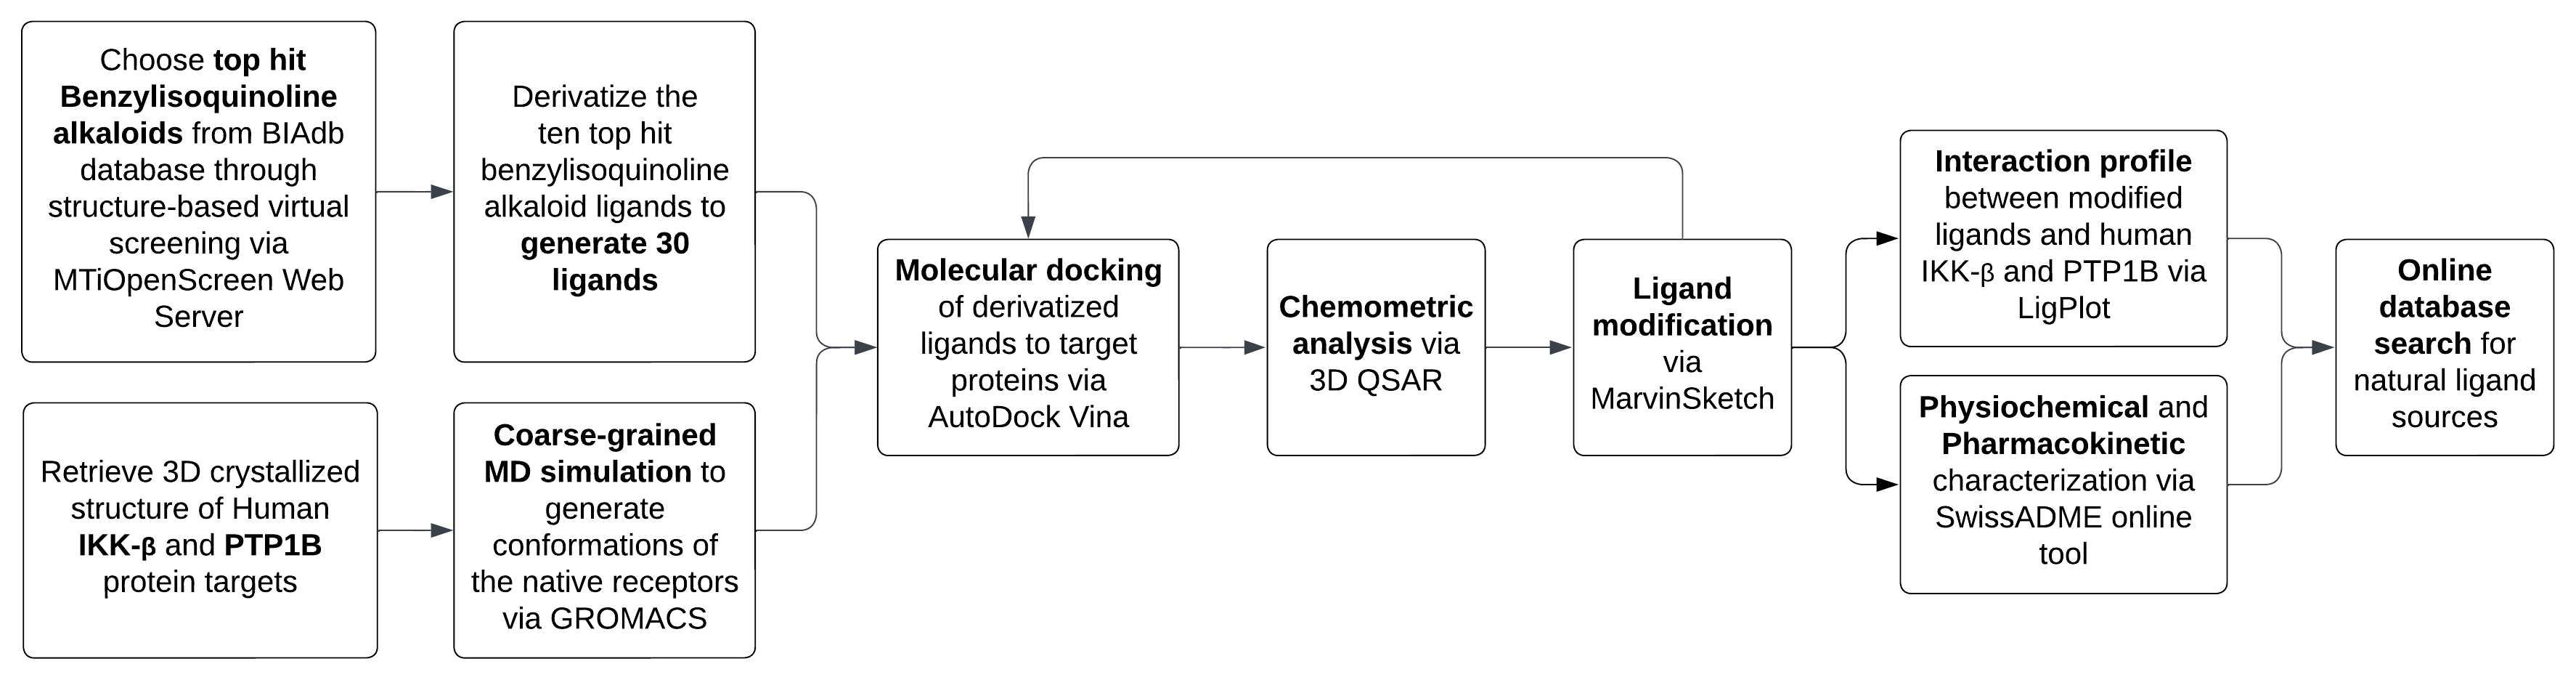
\includegraphics[width=1\linewidth]{Images/Flowchart of Methods.png}
            \caption{Overview of methodology}
            \label{fig:methodology}
        \end{figure}


\section{Initial Ligand Data Set}
Benzylisoquinoline alkaloids targeted for human IKK-$\beta$ and PTP1B  will be filtered and chosen based on lead-likeness (i.e., 250$<$MW$<$350 Da and -4$<$XlogP$<$3.5) and backbone similarity to berberine from the BIadb database. A structure-based virtual screening of the selected benzylisoquinoline alkaloids will be conducted using MTiOpenScreen web server to identify the top 10 ligands against the prepared human IKK-$\beta$ and PTP1B targets.  Each of the ten top hit benzylisoquinoline alkaloid ligands selected from the structure-based virtual screening will be derivatized to obtain 30 ligands for ensemble docking and 3D QSAR analysis. 

\section{Receptor and Ligand Preparation}
The three-dimensional (3D) crystallized structure of human IKK-$\beta$ (PDB ID: \href{https://www.rcsb.org/structure/4KIK}{4KIK}) and PTP1B (PDB ID: \href{https://www.rcsb.org/structure/4I8N}{4I8N}) will be retrieved from the Protein Data Bank, an open access database with 3D protein conformations. Each wild-type receptor will be prepared for subsequent protocols by removing ligand and solvent molecules and adding hydrogen atoms via AutoDock Tools. 

\subsection{Coarse-grained Molecular Dynamics Simulation}
The initial system will be minimized in a vacuum and equilibrated using GROMACS, an open-source software primarily used for biomolecule dynamical simulations. A coarse-grained molecular dynamic (MD) simulation will be run to generate conformations of the native receptors for subsequent ensemble docking. 

Preprocessing of the protein systems will be done by removing heteroatoms. The secondary structures of IKK-$\beta$ and PTP1B will be found and the All-atom models of the systems will be martinized and converted to Coarse grain models using the Martinize python script. As a result, the coarse-grained structures, corresponding topology, and parameter files for the proteins will be generated. Moving on to system preparation for MD simulation, the 'insane' tool to build coarse-grain systems via the 'insane.py' script will be employed to facilitate the solvation and ion addition (i.e., $Na^+$ or $Cl^-$) for system neutrality. 

The Martini 3 force field will be used to unite groups of atoms into effective interaction sites (Paulo et al., 2020). The topology file will be modified to include the parameters required for simulation, incorporating it with the Martini 3 force field. Once the solvated system has been prepared, standard molecular dynamics (MD) simulation protocols will be employed. The energy of the system will be minimized and followed by equilibration. Afterward, a production run of 2$\mu$s will be performed. From the trajectory, an ensemble of PDB files will be extracted via the 'trajout' command wherein the first 10 frames of the trajectory will be included in the file. The resulting pdb file will contain the native conformations of the systems and can initially be visualized using UCSF Chimera.

\section{Ensemble Docking}
The 3D structures of the benzylisoquinoline alkaloid derivatives from 3.0.1 will be obtained from the PubChem Database. Derivatives of the top ten hits will be created and prepared using MarvinSketch. Their geometries will be optimized in Avogadro using the GAFF force field. Afterward, the prepare$_$ligand tool in MGLTools will be used to prepare the compounds for molecular docking to the IKK-$\beta$ and PTP1B ensembles. 

To execute targeted docking, grid box coordinates will be set based on the binding sites of native ligands as predicted by PocketDB and PrankWeb as well as assessments of existing crystal structures. A grid box of 40x40x40 (xyz) and with a 0.375 \r{A} spacing will be used to fully encapsulate the binding sites. AutoDock Vina will be used to predict the ligand-protein interactions. The output is the calculated binding energies and poses for each ligand-target complex based on van der Waals, electrostatic, and hydrogen-bond potentials derived from AMBER force fields. 

\section{3D-QSAR Analysis}
The best resulting pose for each ligand from the molecular docking step will be subjected to chemometric analysis using Open 3D-Align and Open 3D-QSAR. First, Open3D-Align will be used to import the 3D molecular structures of benzylisoquinoline alkaloid ligands and will subsequently be best-aligned. Open 3D-QSAR will then be used to determine the areas favoring or disfavoring functional groups (i.e., steric, electronegative, and electropositive groups) based on non-covalent interactions between the ligand and IKK-$\beta$ and PTP1B respectively. Molecular interaction fields will be computed using AMBER FF99 Van der Waals parameters (steric fields) and a point charge model (electrostatic field). The dataset will be split into training and test sets for later external validation. 

Pretreatment operations will be executed to exclude poorly informative variables that may affect the validity of the model. The following parameters will be met: (1) a grid box with 1.0 \r{A} step size and 5.0 \r{A} outgap; (2) 1.0 x 10$^4$ kcal/mol steric cutoff; (3) 30.0 kcal/mol energy cutoff; zeroing of low energy values ($<$0.05 kcal/mol); (4) exclusion of N-level variables and variables with low standard deviations ($<$0.1); and blocking of unweighted scaling. 

A partial least squares (PLS) model will be built to identify and extract the quantitative influence of specific chemical features of molecules on their biological activity. Cross-validation will be carried out to challenge the internal predictivity of the model (LOO, LTO, LMO). External prediction against the test set will also be used to assess the predictive ability of the model. Moreover, the predictivity may also be improved using fractional factorial design (FFD) variable selection. 

The model's internal and external predictive capability will be validated using the output of cross-validation methods and non-cross-validation methods where q$^2$$>$0.5, r$^2$$>$0.6, and r$^2$pred$>$0.6 with the lowest standard estimation error (SEE). 

The 3D-QSAR model will be visualized with PyMOL. Contour plots representing sterically favored, sterically disfavored, electronegative, and electropositive regions will be used as supporting guides for ligand functionalization. 

\section{Ligand Optimization}
The benzylisoquinoline alkaloid ligands will be modified in MarvinSketch using the results obtained from the 3D-QSAR model. Ligands that demonstrated the highest binding affinities will be used as model ligands when adding substituents. The functionalized compounds will be redocked using the same parameters as in the previous docking step to determine if the structural changes on ligands improved binding affinities to each target receptor.

\section{Protein-ligand interaction analysis}
The interaction profile between the modified benzylisoquinoline alkaloid ligands and human IKK-$\beta$ and PTP1B (e.g. hydrophobic interactions and hydrogen bonds) will be determined by using LigPlot. The presence and strength of intermolecular interactions will be obtained from the generated 2-D schematic representation of the protein-ligand complexes. 

\section{ADME and Toxicity Analysis}
The modified ligands will be subjected to the \href{http://www.swissadme.ch/}{SwissADME} online tool to determine and evaluate their predicted physicochemical and pharmacokinetic characteristics. Such data to be examined include physicochemical properties, lipophilicity, water-solubility, pharmacokinetics, drug-likeliness, and medicinal chemistry to investigate its bioavailability and therapeutic potential (Kumar et al., 2022). Furthermore, \href{https://tox-new.charite.de/protox_II/} {ProToxII} will be used to predict the modified ligands' toxicity in terms of LD50, hepatotoxicity, carcinogenicity, immunotoxicity, mutagenicity, and cytotoxicity. 

\section{Online database Search for natural ligand sources}
The top modified ligand that showed the highest binding affinity and optimal physicochemical and pharmacokinetic characteristics when bound to human IKK-β and PTP1B will be subjected to an online database search to determine if it can be naturally sourced from plants. Specifically, molecules that possess identical structures, which may be primary or secondary metabolites, will be searched. Databases such as the Plant Secondary Compounds Database (\href{https://www.ncbi.nlm.nih.gov/pmc/articles/PMC7924326/}{PSC-db}) and \href{https://www.ncbi.nlm.nih.gov/pmc/articles/PMC4384003/}{Super Natural 3.0} will be utilized.  

\pagebreak

\chapter{Others}

\section{Line-Item Budget}

% \usepackage{tabularray}
\begin{table}[h]
\centering
\begin{tblr}{
  cell{2}{2} = {r},
  cell{3}{2} = {r},
  cell{4}{2} = {r},
  cell{5}{2} = {r},
  cell{6}{2} = {r},
  cell{7}{2} = {r},
  cell{8}{2} = {r},
  cell{9}{2} = {r},
  cell{10}{2} = {r},
  cell{11}{2} = {r},
  hline{1-2,11-12} = {-}{},
}
\textbf{Item/Service}                    & \textbf{Estimated Cost (in PHP)} \\
\textbf{Computational Resources}         &                                  \\
~ ~ ~Electricity                         & 2,000                            \\
~ ~ ~Internet                            & 3,800                            \\
~ ~ ~Data storage for data backup        & 500                              \\
\textbf{Communication and Collaboration} & 500                              \\
\textbf{Transportation}                  & 1,500                            \\
\textbf{Miscellaneous}                   &                                  \\
~ ~ ~Administrative fees                 & 1,000                            \\
~ ~ ~Contingency fund                    & 1,000                            \\
\textbf{TOTAL}                           & \textbf{10,300}                  
\end{tblr}
\end{table}

\section{Gantt Chart}

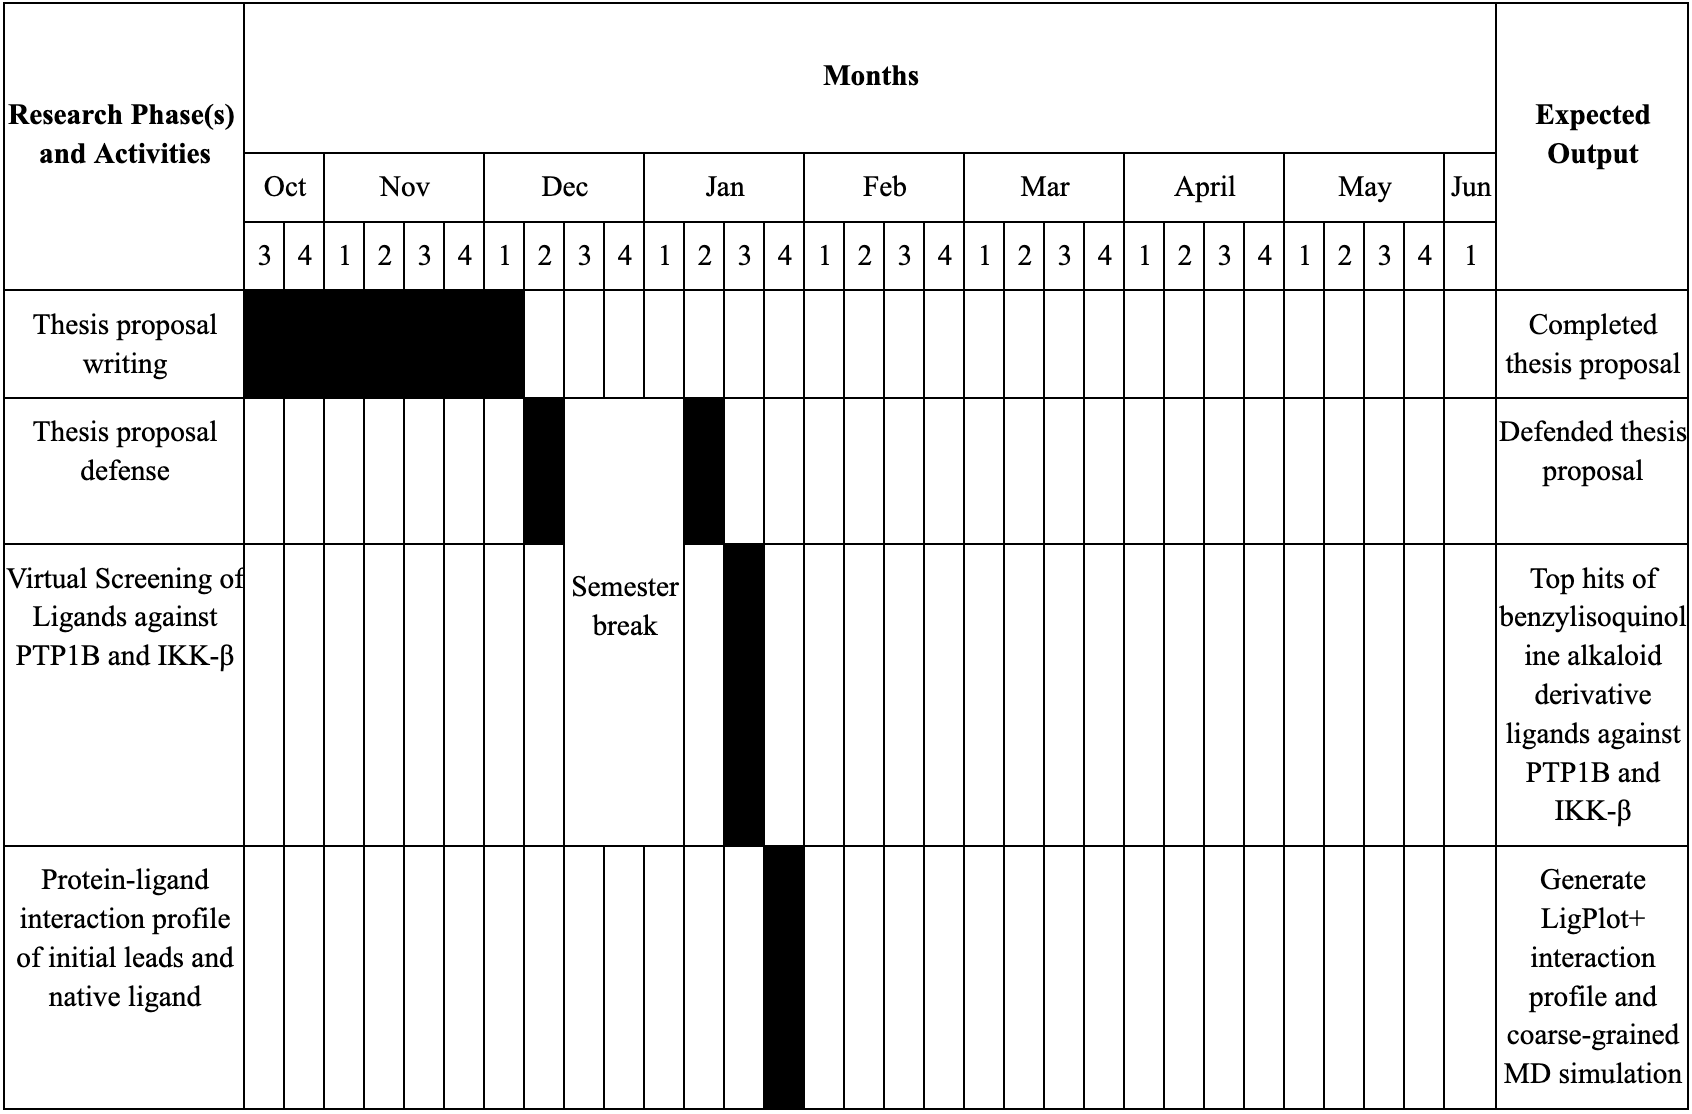
\includegraphics[width=1\textwidth, center]{Images/GANTT 1.png}

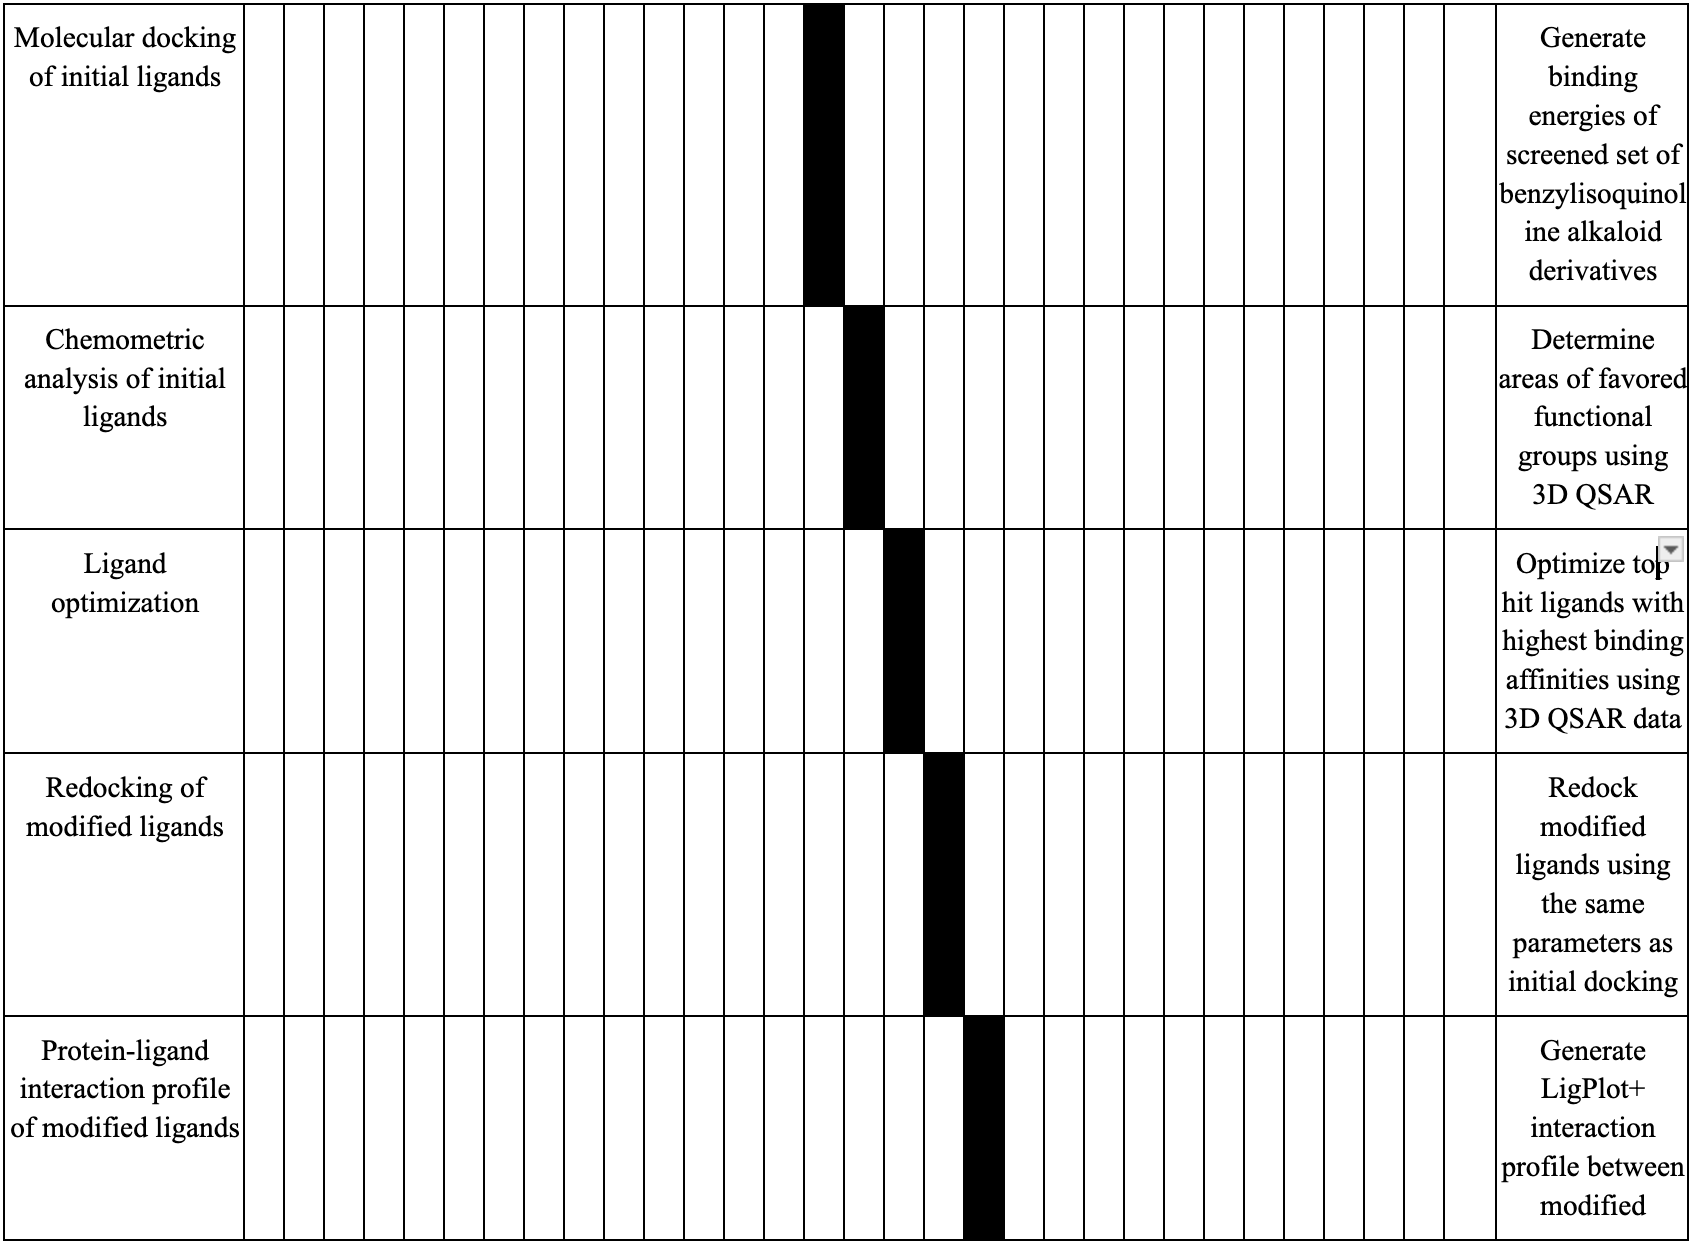
\includegraphics[width=1\textwidth, center]{Images/GANTT 2.png}

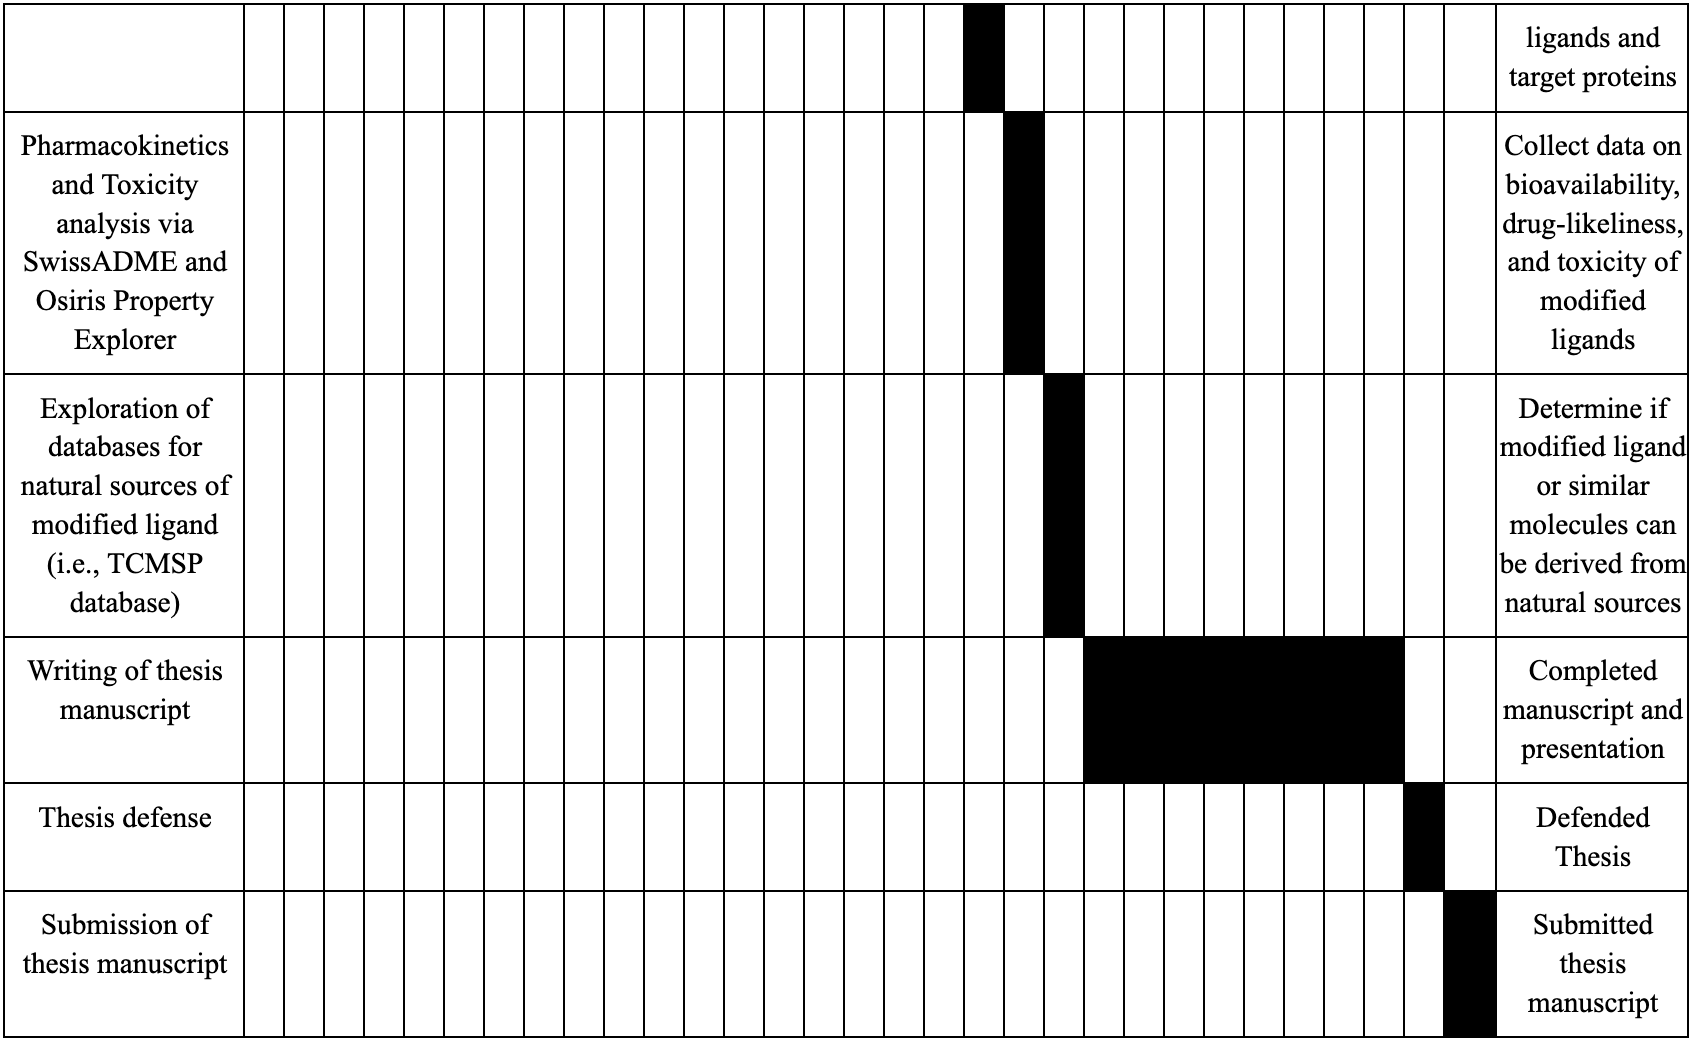
\includegraphics[width=1\textwidth, center]{Images/GANTT 3.png}

\pagebreak

\end{document}
